\documentclass[11pt,a4paper]{article}
\usepackage[utf8]{inputenc}
\usepackage[italian]{babel}
\usepackage{geometry}
\usepackage{graphicx}
\usepackage{float}
\usepackage{tabularx}
\usepackage{booktabs}
\usepackage{hyperref}
\usepackage{fancyhdr}
\usepackage{lastpage}
\usepackage{longtable}

\geometry{margin=2.5cm}

% Intestazione e piè di pagina
\pagestyle{fancy}
\fancyhf{}
\renewcommand{\headrulewidth}{0pt}
\fancyfoot[C]{\thepage\ di \pageref{LastPage}}

\begin{document}

% Prima pagina - Intestazione
\begin{titlepage}
    \centering
    
    % Logo Università
    \begin{figure}[H]
        \centering
        
\includegraphics[width=0.3\textwidth]{../logoUnipd.jpg}
    \end{figure}
    
    \vspace{0.5cm}
    
    \textbf{\Large Università degli Studi di Padova} \\
    \vspace{0.2cm}
    \textbf{Laurea in Informatica} \\
    \vspace{0.2cm}
    \textbf{Corso di Ingegneria del Software} \\
    \vspace{0.2cm}
    \textbf{Anno Accademico 2025/2026} \\
    
    \vspace{1cm}
    
    % Logo gruppo
    \begin{figure}[H]
        \centering
        
\includegraphics[width=0.2\textwidth]{../LogoByteMe.jpg}
    \end{figure}
    
    \vspace{0.5cm}
    
    \textbf{\Large Gruppo ByteMe} \\
    \vspace{0.2cm}
    \texttt{byteme2025swe@gmail.com} \\
    
    \vspace{1cm}
    
    \textbf{\Huge Analisi dei Requisiti} \\
    
    \vspace{1.5cm}
    
    \begin{table}[H]
        \centering
        \begin{tabular}{|l|p{5cm}|}
            \hline
            \textbf{Versione} & 0.5.1 \\
            \hline
            \textbf{Stato} & In corso \\
            \hline
            \textbf{Redazione} & Tutto il gruppo \\
            \hline
            \textbf{Verifica} & Tutto il gruppo \\
            \hline
            \textbf{Approvazione} & Tutto il gruppo \\
            \hline
            \textbf{Proprietario} & ByteMe \\
            \hline
            \textbf{Uso} & Esterno \\
            \hline
            \textbf{Destinatari} & Prof. Tullio Vardanega \\ & Prof. Riccardo Cardin \\
            \hline
        \end{tabular}
    \end{table}
    
    \vfill
\end{titlepage}

% Seconda pagina - Versionamento
\thispagestyle{empty}
\section*{Registro dei Cambiamenti}

\begin{longtable}[H]{|c|c|c|>{\raggedright\arraybackslash}p{0.3\textwidth}|c|}
    \caption{Registro delle versioni del documento}
    \label{tab:versionamento} \\
        \hline
        \textbf{Versione} & \textbf{Data} & \textbf{Autore} & \textbf{Descrizione} & \textbf{Verifica} \\
        \hline
        0.5.1 & 05/02/2026 & Joseph Grant & Macroarea 2, modifica UC 2.1.* e relativi requisiti &  \\
        \hline
        0.5.0 & 01/02/2026 & Joseph Grant & Aggiunta casi d'uso macroarea 5 &  \\
        \hline
        0.4.9 & 30/01/2026 & Joseph Grant & Correzioni requisiti inerenti alla macroarea 4 &  \\
        \hline
        0.4.8 & 29/01/2026 & Joseph Grant & Correzioni requisiti inerenti alla macroarea 3 &  \\
        \hline
        0.4.7 & 28/01/2026 & Joseph Grant & Aggiunta requisiti inerenti alla macroarea 2 &  \\
        \hline
        0.4.6 & 27/01/2026 & Joseph Grant & Correzione requisiti macroarea 1 &  \\
        \hline
        0.4.5 & 27/01/2026 & Joseph Grant & Aggiunta requisiti inerenti alla macroarea 1 &  \\
        \hline
        0.4.4 & 21/01/2026 & Joseph Grant & Aggiunta requisiti dal doc FIX REQUISITI &  \\
        \hline
        0.4.3 & 19/01/2026 & Joseph Grant & Fix diagrammi &  \\
        \hline
        0.4.2 & 17/01/2026 & Giulia Barzon & Fix area 5 e diagrammi & Joseph Grant \\
        \hline
        0.4.1 & 17/01/2026 & Elisa Marchioro & Fix nomi casi d'uso & Joseph Grant \\
        \hline
        0.4.0 & 17/01/2026 & Elisa Marchioro & Sistemata macroarea 3 e 4 e relativi diagrammi & Joseph Grant \\
        \hline
        0.3.9 & 15/01/2026 & Giulia Barzon & Aggiunti diagrammi macroarea 1 e 2 & Joseph Grant \\
        \hline
        0.3.8 & 15/01/2026 & Giulia Barzon & Sistemati casi ed estensioni macroarea 2 & Joseph Grant \\
        \hline
        0.3.7 & 15/01/2026 & Joseph Grant & Sistemate estensioni macroarea 1 e sistemato UC 3.0 & Giulia Barzon\\
        \hline
        0.3.6 & 12/01/2026 & Matteo Cuogo & Estensione e correzione casi d'uso macroarea 1 & Joseph Grant\\
        \hline
        0.3.5 & 09/01/2026 & Giulia Barzon & Corretti UC 1.1, 3.1, 3.2 & Joseph Grant\\
        \hline
        0.3.4 & 04/01/2026 & Tommaso Tombacco & Correzione requisiti macroarea 2 & Elisa Marchioro\\
        \hline
        0.3.3 & 02/01/2026 & Elisa Marchioro & Aggiunti requisiti macroarea 4 &  Matteo Cuogo\\
        \hline
        0.3.2 & 01/01/2026 & Tommaso Tombacco & Piccole correzioni & Matteo Cuogo\\
        \hline
        0.3.1 & 01/01/2026 & Joseph Grant & Piccole correzioni e aggiunte &  Matteo Cuogo\\
        \hline
        0.3.0 & 30/12/2025 & Giulia Barzon & Correzione requisiti macroarea 1 e inserimento diagrammi completi & Matteo Cuogo \\
        \hline
        0.2.3 & 29/12/2025 & Giulia Barzon & Aggiunti primi diagrammi casi d'uso &  Matteo Cuogo \\
        \hline
        0.2.2 & 29/12/2025 & Giulia Barzon & Rimosso vecchio caso d'uso 3.3 per incoerenza e sistemati relativi requisiti & Matteo Cuogo \\
        \hline
        0.2.1 & 29/12/2025 & Tommaso Tombacco & Modifiche ad alcuni casi d'uso &  Matteo Cuogo\\ 
        \hline
        0.2.0 & 28/12/2025 & Joseph Grant & Aggiunta dei requisiti macroarea 1, 2, 3 e 5 &  Matteo Cuogo\\ 
        \hline
        0.1.6 & 27/12/2025 & Elisa Marchioro & Aggiunto sottocaso 4.3.1 & Matteo Cuogo\\ 
        \hline
        0.1.5 & 27/12/2025 & Joseph Grant & Aggiunta sezione 'verifica' al versionamento & Elisa Marchioro\\ 
        \hline
        0.1.4 & 27/12/2025 & Matteo Cuogo & Correzione e ampliamento dei casi d'uso rivisti & Elisa Marchioro\\
        \hline
        0.1.3 & 14/12/2025 & Giulia Barzon & Correzione errori e scrittura introduzione e classificazione dei requisiti & Elisa Marchioro\\
        \hline
        0.1.2 & 08/12/2025 & Giulia Barzon & Inserimento caso d'uso 1.9 (Unicode) e creazione primo diagramma caso d'uso di esempio (2.3 e 2.9-2.11) & Elisa Marchioro\\
        \hline
        0.1.0 & 07/12/2025 & Giulia Barzon & Inserimeno casi d'uso identificati & Elisa Marchioro\\
        \hline
        0.0.1 & 20/11/2025 & Giulia Barzon & Creazione del documento e scrittura introduzione & Elisa Marchioro\\
        \hline
\end{longtable}

\newpage

% Terza pagina - Indice
\tableofcontents
\thispagestyle{empty}
\newpage

% Dalla quarta pagina - Contenuto principale
\setcounter{page}{1}

\section{Introduzione}
\subsection{Scopo del documento}
Questo documento descrive l'analisi dei requisiti per il progetto \textbf{"Second Brain"}. Il documento definisce in modo dettagliato i casi d'uso e i requisiti del sistema, che combina un editor di testo Markdown con funzionalità AI avanzate per assistere gli utenti nella creazione, revisione e miglioramento dei contenuti testuali.

L'obiettivo principale è fornire una specifica completa delle funzionalità che il sistema deve implementare, classificando i requisiti in obbligatori, desiderabili e opzionali, in linea con le richieste della proponente Zucchetti.

\subsection{Glossario}
Per evitare ambiguità, i termini tecnici usati nel documento vengono definiti in modo più approfondito nel documento "Glossario" che si trova nella repository del gruppo nella cartella "Documenti\textunderscore interni".

I termini che vengono considerati meritevoli di approfondimenti sono indicati con una G a pedice.

\subsection{Riferimenti}
\subsubsection{Riferimenti normativi}
\begin{itemize}
    \item Norme di Progetto - Documento interno del gruppo ByteMe
    \item Regolamento del progetto didattico
\end{itemize}

\subsubsection{Riferimenti informativi}
\begin{itemize}
    \item Capitolato C6 "Second Brain", Zucchetti
    \item Slide del corso di Ingegneria del Software
    \item Verbali interni ed esterni
\end{itemize}

\newpage

\section{Descrizione del progetto}
\subsection{Obiettivi del prodotto}
Il progetto \textbf{Second Brain} si propone di rivoluzionare il processo di scrittura e organizzazione delle idee attraverso l'integrazione di Large Language Models\textsubscript{G} in un editor di testo moderno. Gli obiettivi principali sono:

\begin{itemize}
    \item Fornire uno strumento di \textit{note-taking} avanzato che combini la semplicità del Markdown\textsubscript{G} con la potenza dell'IA generativa.
    \item Implementare un sistema di \textit{critica intelligente} del testo basato sulla metodologia dei "Sei Cappelli per Pensare" di Edward De Bono.
    \item Semplificare il processo di scrittura attraverso funzionalità di correzione, rielaborazione, traduzione e ottimizzazione automatica del testo.
    \item Implementare un sistema di \textit{distant writing} che permette di generare un testo completo a partire da un breve prompt dell'utente.
\end{itemize}


\subsection{Funzionalità del prodotto}
Il sistema offre le seguenti funzionalità principali:

\begin{itemize}
    \item \textbf{Editor Markdown\textsubscript{G}} avanzato con anteprima in tempo reale
    \item \textbf{Integrazione LLM\textsubscript{G}} per operazioni su testo selezionato o completo
    \item \textbf{Comandi base di elaborazione}: riassunto, riscrittura, traduzione, correzione grammaticale
    \item \textbf{Sistema di critica testuale} basato sui 6 cappelli per pensare
    \item \textbf{Distant Writing\textsubscript{G}} per generazione guidata di contenuti
    \item \textbf{Persistenza dati} con salvataggio locale e opzionale su cloud
\end{itemize}

\subsection{Caratteristiche del prodotto}
Le caratteristiche distintive che rendono unico il prodotto sono:

\begin{itemize}
    \item \textbf{Architettura ibrida}: applicazione web con possibile estensione server-side
    \item \textbf{Interfaccia semplice}: design pulito per un editor chiaro e semplice e anteprima in tempo reale
    \item \textbf{Multi-piattaforma}: accessibile da qualsiasi browser moderno
    \item \textbf{Estensibilità}: architettura modulare che permette l'aggiunta di nuove funzionalità
    
\end{itemize}

\subsection{Utenti}
Il prodotto è rivolto alle seguenti categorie di utenti:

\begin{itemize}
    \item \textbf{Studenti}: per la stesura di appunti, riassunti e materiale di studio
    \item \textbf{Professionisti}: per la creazione di documenti aziendali, report e presentazioni
    \item \textbf{Scrittori e content creator}: per l'ideazione, stesura e revisione di contenuti
    \item \textbf{Ricercatori}: per l'organizzazione di appunti di ricerca e letteratura
    \item \textbf{Utenti generici}: chiunque abbia bisogno di un editor per esigenze di scrittura assistita
\end{itemize}

Non sono richieste competenze tecniche avanzate per l'utilizzo delle funzionalità base, rendendo il prodotto accessibile a un'ampia gamma di utenti.

\newpage

\section{Casi d'uso}
\subsection{Introduzione}
Questa sezione descrive in dettaglio i casi d'uso del sistema \textbf{Second Brain}, identificando tutte le interazioni significative tra gli attori e il sistema. Il gruppo ha deciso di suddividere i casi d'uso in macroaree per organizzare in modo più chiaro i casi d'uso individuati. Ogni caso d'uso è definito attraverso:

\begin{itemize}
    \item \textbf{Codice identificativo} univoco seguendo lo schema UC-X.Y
    \item \textbf{Descrizione} chiara e concisa dello scenario
    \item \textbf{Attori} coinvolti nell'interazione
    \item \textbf{Precondizioni} necessarie per l'esecuzione
    \item \textbf{Postcondizioni} risultanti dall'esecuzione
    \item \textbf{Scenario principale} con sequenza di passi
\end{itemize}

I casi d'uso sono organizzati per macroaree funzionali per facilitare la lettura e il tracciamento.

\subsection{Attori}
Il sistema prevede i seguenti attori:

\begin{itemize}
    \item \textbf{Utente Non Autenticato\textsubscript{G}}: utente che accede alle funzionalità base senza registrazione
    \item \textbf{Utente Autenticato\textsubscript{G}}: utente registrato che accede alle funzionalità avanzate e alla persistenza cloud
    \item \textbf{Sistema AI\textsubscript{G}}: componente di intelligenza artificiale che elabora le richieste testuali
    \item \textbf{Sistema di Persistenza\textsubscript{G}}: componente responsabile del salvataggio e recupero dei dati
\end{itemize}

L'attore principale è l'\textbf{Utente} (nelle sue due varianti), mentre gli altri attori sono considerati secondari e interagiscono con il sistema in modo trasparente all'utente finale.

\newpage

\subsection{Macroarea 1 - Editor di testo}
\subsubsection{UC-1.0 - Modifica del testo tramite sintassi markdown}
\begin{itemize}
    \item \textbf{Attore principale}: Utente generico
    \item \textbf{Descrizione}: L’utente scrive nell’apposita area di testo utilizzando la sintassi markdown
    \item \textbf{Precondizioni}: L’area di testo è vuota o riempita parzialmente
    \item \textbf{Postcondizioni}: L’area di testo contiene le modifiche fatte dall’utente
    \item \textbf{Scenario principale}:
        \begin{itemize}
            \item L’utente si posiziona sull’area di testo
            \item L’utente inserisce testo rispettando la sintassi markdown
        \end{itemize}
    \item \textbf{Estensioni}:
        \begin{itemize}
            \item La connessione Internet viene persa durante la digitazione
            \item L'editor non risponde ai comandi
        \end{itemize}
\end{itemize}

\subsubsection{UC-1.0.1 - Gestione perdita della connesione Internet}
\begin{itemize}
    \item \textbf{Attore principale}: Utente generico
    \item \textbf{Descrizione}: L'utente sta digitando testo e la connessione internet si interrompe
    \item \textbf{Precondizioni}: L'utente sta digitando testo nell'editor
    \item \textbf{Postcondizioni}: Il sistema informa l'utente e si sincronizza quando la connessione ritorna disponibile
    \item \textbf{Scenario principale}:
        \begin{itemize}
            \item L'utente sta digitando testo nell'editor
            \item La connessione Internet si interrompe
            \item Il sistema informa l'utente con un messaggio
            \item Quando la connessione ritorna disponibile, il sistema sincronizza i dati con il server
        \end{itemize}
\end{itemize}

\subsubsection{UC-1.0.2 - Gestione mancante risposta dell'editor}
\begin{itemize}
    \item \textbf{Attore principale}: Utente generico
    \item \textbf{Descrizione}: L'utente sta digitando testo e l'editor non risponde
    \item \textbf{Precondizioni}: L'utente sta digitando testo nell'editor
    \item \textbf{Postcondizioni}: Il sistema informa l'utente e mostra un messaggio di errore
    \item \textbf{Scenario principale}:
        \begin{itemize}
            \item L'utente sta digitando testo nell'editor
            \item L'editor non risponde
            \item Il sistema informa l'utente con un messaggio
        \end{itemize}
\end{itemize}

\begin{figure}[H]
    \centering
    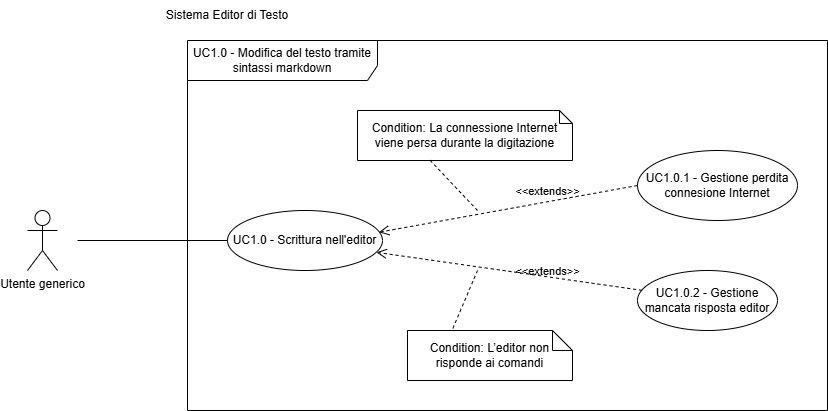
\includegraphics[width=0.8\textwidth]{../UCimg/UC1.0.jpg}
    \caption{Diagramma dei casi d'uso UC-1.0, 1.0.1, 1.0.2}
    \label{fig:uc1.0}
\end{figure}

\subsubsection{UC-1.1 - Visualizzazione anteprima in tempo reale}
\begin{itemize}
    \item \textbf{Attore principale}: Utente generico
    \item \textbf{Descrizione}: Visualizzazione in tempo reale del testo formattato
    \item \textbf{Precondizioni}: L'editor contiene testo con sintassi Markdown
    \item \textbf{Postcondizioni}: Viene visualizzata l'anteprima formattata del testo in un'area apposita
    \item \textbf{Scenario principale}:
        \begin{itemize}
            \item L'utente modifica il testo nell'editor
            \item Il sistema elabora la sintassi Markdown
            \item Il sistema aggiorna il pannello di preview mostrando l’anteprima formattata del documento
            \item L'utente può confrontare editing e risultato finale
        \end{itemize}
    \item \textbf{Estensioni}:
        \begin{itemize}
            \item L'anteprima non si aggiorna correttamente
        \end{itemize}
\end{itemize}

\subsubsection{UC-1.1.1 - Gestione errore nell'anteprima}
\begin{itemize}
    \item \textbf{Attore principale}: Utente generico
    \item \textbf{Descrizione}: L'utente ha scritto del testo ma la sezione di anteprima non si aggiorna correttamente
    \item \textbf{Precondizioni}: L'utente ha scritto del testo
    \item \textbf{Postcondizioni}: Il sistema informa l'utente e mostra un messaggio di errore
    \item \textbf{Scenario principale}:
        \begin{itemize}
            \item L'utente sta digitando testo nell'editor
            \item La sezione di anteprima non si aggiorna correttamente
            \item Il sistema informa l'utente con un messaggio di errore
        \end{itemize}
\end{itemize}

\begin{figure}[H]
    \centering
    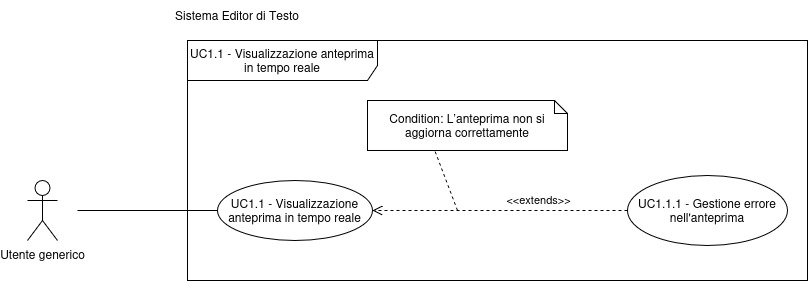
\includegraphics[width=0.8\textwidth]{../UCimg/UC1.1.jpg}
    \caption{Diagramma dei casi d'uso UC-1.1, 1.1.1}
    \label{fig:uc1.1}
\end{figure}

\subsubsection{UC-1.2 - Selezione del testo}
\begin{itemize}
    \item \textbf{Attore principale}: Utente generico
    \item \textbf{Descrizione}: Selezione di porzioni di testo nell’editor
    \item \textbf{Precondizioni}: È presente testo nell'editor
    \item \textbf{Postcondizioni}: Una porzione di testo viene selezionata dall’utente
    \item \textbf{Scenario principale}:
        \begin{itemize}
            \item L'utente evidenzia una porzione di testo con mouse o tastiera
        \end{itemize}
\end{itemize}

\begin{figure}[H]
    \centering
    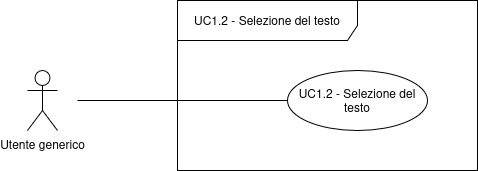
\includegraphics[width=0.8\textwidth]{../UCimg/UC1.2.jpg}
    \caption{Diagramma dei casi d'uso UC-1.2}
    \label{fig:uc1.2}
\end{figure}

\subsubsection{UC-1.3 - Copiare il testo}
\begin{itemize}
    \item \textbf{Attore principale}: Utente generico
    \item \textbf{Descrizione}: L'utente copia una parte di testo dall'area di modifica testo
    \item \textbf{Precondizioni}: Testo presente e selezionato
    \item \textbf{Postcondizioni}: L'utente ha copiato il testo da lui selezionato
    \item \textbf{Scenario principale}:
        \begin{itemize}
            \item L'utente seleziona una porzione di testo
            \item L'utente utilizza il comando "Copia" tramite:
                \begin{enumerate}
                    \item Tasto di scelta rapida (Ctrl+C)
                    \item Menu contestuale (tasto destro)
                    \item Toolbar dell'editor
                \end{enumerate}
            \item Il testo selezionato viene copiato negli appunti di sistema
            \item Il sistema manda un messaggio di successo
        \end{itemize}
\end{itemize}

\subsubsection{UC-1.4 - Incollare il testo}
\begin{itemize}
    \item \textbf{Attore principale}: Utente generico
    \item \textbf{Descrizione}: L'utente incolla una parte di testo nell'area di modifica testo
    \item \textbf{Precondizioni}: Testo presente negli appunti di sistema
    \item \textbf{Postcondizioni}: L'utente ha incollato il testo precedentemente copiato
    \item \textbf{Scenario principale}:
        \begin{itemize}
            \item L'utente posiziona il cursore nel punto desiderato
            \item L'utente utilizza il comando "Incolla" tramite:
                \begin{enumerate}
                    \item Tasto di scelta rapida (Ctrl+V)
                    \item Menu contestuale (tasto destro)
                    \item Toolbar dell'editor (opzionale)
                \end{enumerate}
            \item Il testo dagli appunti viene inserito nella posizione del cursore
        \end{itemize}
\end{itemize}

\subsubsection{UC-1.5 - Tagliare il testo}
\begin{itemize}
    \item \textbf{Attore principale}: Utente generico
    \item \textbf{Descrizione}: L'utente taglia una parte di testo dall'area di modifica, rimuovendola dal documento e copiandola negli appunti
    \item \textbf{Precondizioni}: Testo presente e selezionato
    \item \textbf{Postcondizioni}: Il testo selezionato viene rimosso dall'editor e salvato negli appunti di sistema
    \item \textbf{Scenario principale}:
        \begin{itemize}
            \item L'utente seleziona una porzione di testo
            \item L'utente utilizza il comando "Taglia" tramite:
                \begin{enumerate}
                    \item Tasto di scelta rapida (Ctrl+X)
                    \item Menu contestuale (tasto destro)
                    \item Toolbar dell'editor (opzionale)
                \end{enumerate}
            \item Il sistema rimuove il testo selezionato dall'editor
            \item Il testo rimosso viene salvato negli appunti di sistema
            \item Il sistema manda un messaggio di successo
        \end{itemize}
\end{itemize}

\begin{figure}[H]
    \centering
    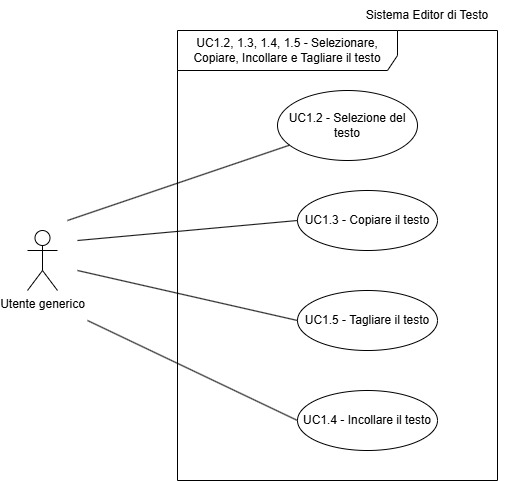
\includegraphics[width=0.8\textwidth]{../UCimg/UC1.3_1.5.jpg}
    \caption{Diagramma dei casi d'uso UC-1.3, 1.4, 1.5}
    \label{fig:uc1.3}
\end{figure}

\subsubsection{UC-1.6 - Annullamento modifica (Undo)}
\begin{itemize}
    \item \textbf{Attore principale}: Utente generico
    \item \textbf{Descrizione}: Annullamento dell'ultima operazione di modifica effettuata
    \item \textbf{Precondizioni}: È stata effettuata almeno una modifica al testo e l'utente desidera annullare l'ultima operazione eseguita
    \item \textbf{Postcondizioni}: Il testo ritorna allo stato precedente l'ultima modifica
    \item \textbf{Scenario principale}:
        \begin{itemize}
            \item L'utente effettua una modifica al testo che non soddisfa le sue aspettative
            \item L'utente seleziona l'opzione "Annulla" tramite:
                \begin{enumerate}
                    \item Tasto di scelta rapida (Ctrl+Z)
                    \item Pulsante nella toolbar dell'editor (freccia verso sinistra)
                \end{enumerate}
            \item Il sistema ripristina il testo allo stato precedente la modifica
            \item L'operazione annullata viene spostata nella coda redo
        \end{itemize}
    \item \textbf{Estensioni}:
        \begin{itemize}
            \item Non ci sono operazioni da annullare
        \end{itemize}
\end{itemize}

\subsubsection{UC-1.6.1 - L'utente non ha effettuato modifiche anullabili}
\begin{itemize}
    \item \textbf{Attore principale}: Utente generico
    \item \textbf{Descrizione}: L'utente tenta di annullare un'operazione quando non ci sono modifiche anullabili
    \item \textbf{Precondizioni}: L'utente non ha effettuato modifiche anullabili
    \item \textbf{Postcondizioni}: Il documento rimane invariato
    \item \textbf{Scenario principale}:
        \begin{itemize}
            \item L'utente tenta di selezionare l'opzione "Annulla"
            \item Il sistema informa l'utente con un messaggio
            \item Il comando undo non modifica il documento
        \end{itemize}
\end{itemize}

\subsubsection{UC-1.7 - Ripristino modifica (Redo)}
\begin{itemize}
    \item \textbf{Attore principale}: Utente generico
    \item \textbf{Descrizione}: Ripristino di un'operazione precedentemente annullata
    \item \textbf{Precondizioni}: È stata effettuata almeno un'operazione di undo; l'utente desidera ripristinare un'operazione precedentemente annullata
    \item \textbf{Postcondizioni}: Il testo ritorna allo stato successivo all'operazione ripristinata
    \item \textbf{Scenario principale}:
        \begin{itemize}
            \item L'utente ha annullato una o più operazioni con undo
            \item L'utente decide di ripristinare un'operazione annullata
            \item L'utente seleziona l'opzione "Ripristina" tramite:
                \begin{enumerate}
                    \item Tasto di scelta rapida (Ctrl+Y o Ctrl+Shift+Z)
                    \item Pulsante nella toolbar dell'editor
                \end{enumerate}
            \item Il sistema riapplica l'ultima operazione annullata
            \item L'operazione viene rimossa dalla coda redo
        \end{itemize}
    \item \textbf{Estensioni}:
        \begin{itemize}
            \item Non ci sono operazioni da ripristinare
        \end{itemize}
\end{itemize}

\subsubsection{UC-1.7.1 - Errore per modifiche non ripristinabili}
\begin{itemize}
    \item \textbf{Attore principale}: Utente generico
    \item \textbf{Descrizione}: L'utente tenta di ripristinare un'operazione quando non ci sono modifiche ripristinabili
    \item \textbf{Precondizioni}: L'utente non ha effettuato modifiche ripristinabili
    \item \textbf{Postcondizioni}:  Il documento rimane invariato
    \item \textbf{Scenario}:
        \begin{itemize}
            \item L'utente tenta di selezionare l'opzione "Ripristina"
            \item Il sistema informa l'utente con un messaggio
            \item Il comando redo non modifica il documento
        \end{itemize}
\end{itemize}

\begin{figure}[H]
    \centering
    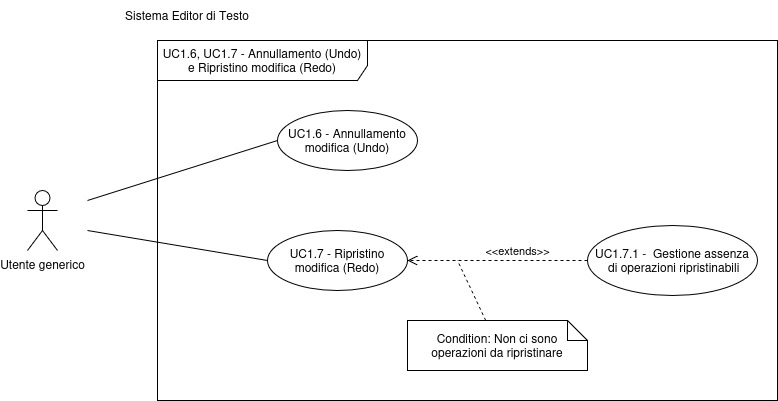
\includegraphics[width=0.8\textwidth]{../UCimg/UC1.6_1.7.jpg}
    \caption{Diagramma dei casi d'uso UC-1.6, 1.7 e estensioni}
    \label{fig:uc1.6}
\end{figure}

\subsubsection{UC-1.8.0 - Modifica del testo selezionato tramite barra degli strumenti}
\begin{itemize}
    \item \textbf{Attore principale}: Utente generico
    \item \textbf{Descrizione}: Formattazione del testo selezionato tramite la barra degli strumenti dell'editor
    \item \textbf{Precondizioni}: È presente testo nell'editor
    \item \textbf{Postcondizioni}: Il testo selezionato viene formattato secondo la sintassi Markdown
    \item \textbf{Scenario principale}:
        \begin{itemize}
            \item L'utente seleziona il testo da formattare
            \item L'utente clicca sul pulsante desiderato nella barra degli strumenti
            \item Il sistema applica automaticamente la sintassi Markdown corrispondente al testo selezionato
            \item Il testo formattato viene visualizzato nell'area di anteprima
        \end{itemize}
    \item \textbf{Estensioni}:
        \begin{itemize}
            \item Combinazione di più formattazioni diverse
            \item Il testo ha già una specifica formattazione e l'utente la applica di nuovo
            \item Selezione di testo che è parzialmente formattato
        \end{itemize}
\end{itemize}

\subsubsection{UC-1.8.0.1 - Gestione combinazioni di più formattazioni diverse}
\begin{itemize}
    \item \textbf{Attore principale}: Utente generico
    \item \textbf{Descrizione}: L'utente tenta di applicare una formattazione a un testo che ha già una formattazione
    \item \textbf{Precondizioni}: Il testo selezionato ha già una formattazione
    \item \textbf{Postcondizioni}: Il sistema applica la nuova formattazione sopra alla formattazione esistente, senza eliminarla
    \item \textbf{Scenario principale}:
        \begin{itemize}
            \item L'utente seleziona del testo già formattato
            \item L'utente clicca sul pulsante della nuova formattazione nella toolbar
            \item Il sistema applica la nuova formattazione al testo selezionato in aggiunta alla formattazione esistente
        \end{itemize}
\end{itemize}

\subsubsection{UC-1.8.0.2 - Rimozione formattazione}
\begin{itemize}
    \item \textbf{Attore principale}: Utente generico
    \item \textbf{Descrizione}: L'utente riapplica la stessa formattazione a una porzione di testo
    \item \textbf{Precondizioni}: Il testo selezionato è formattato
    \item \textbf{Postcondizioni}: Il testo perde quella formattazione
    \item \textbf{Scenario principale}:
        \begin{itemize}
            \item L'utente seleziona il testo formattato
            \item L'utente clicca sul pulsante della stessa formattazione nella toolbar
            \item Il sistema rimuove la formattazione dal testo selezionato
        \end{itemize}
\end{itemize}

\subsubsection{UC-1.8.0.3 - Gestione testo già parzialmente formattato}
\begin{itemize}
    \item \textbf{Attore principale}: Utente generico
    \item \textbf{Descrizione}: L'utente applica la stessa formattazione a una porzione del testo che contiene parzialmente la stessa formattazione
    \item \textbf{Precondizioni}: Il testo selezionato è parzialmente formattato
    \item \textbf{Postcondizioni}: Il testo viene formattato per intero
    \item \textbf{Scenario principale}:
        \begin{itemize}
            \item L'utente seleziona del testo
            \item Il testo selezionato è parzialmente formattato
            \item L'utente clicca sul pulsante della stessa formattazione nella toolbar
            \item Il sistema applica la formattazione a tutto il testo selezionato
        \end{itemize}
\end{itemize}

\begin{figure}[H]
    \centering
    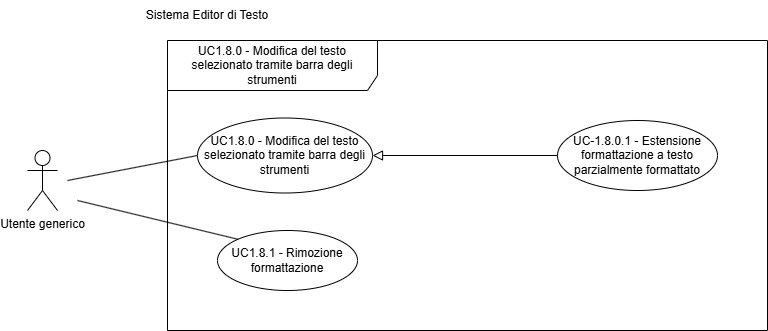
\includegraphics[width=0.8\textwidth]{../UCimg/UC1.8.0.1.jpg}
    \caption{Diagramma dei casi d'uso UC-1.8.0, 1.8.0.1, 1.8.0.2, 1.8.0.3}
    \label{fig:uc1.8.0}
\end{figure}

\subsubsection{UC-1.8.1 - Applicazione grassetto al testo selezionato}
\begin{itemize}
    \item \textbf{Attore principale}: Utente generico
    \item \textbf{Descrizione}: Formattazione del testo selezionato in grassetto tramite barra degli strumenti
    \item \textbf{Precondizioni}: È presente testo selezionato nell'editor
    \item \textbf{Postcondizioni}: Il testo selezionato viene formattato in grassetto
    \item \textbf{Scenario principale}:
        \begin{itemize}
            \item L'utente seleziona il testo da rendere in grassetto
            \item L'utente clicca sul pulsante "Grassetto" nella toolbar
            \item Il sistema applica la sintassi Markdown per il grassetto
            \item Il testo viene visualizzato in grassetto nell'anteprima
        \end{itemize}
\end{itemize}

\subsubsection{UC-1.8.2 - Applicazione corsivo al testo selezionato}
\begin{itemize}
    \item \textbf{Attore principale}: Utente generico
    \item \textbf{Descrizione}: Formattazione del testo selezionato in corsivo tramite barra degli strumenti
    \item \textbf{Precondizioni}: È presente testo selezionato nell'editor
    \item \textbf{Postcondizioni}: Il testo selezionato viene formattato in corsivo
    \item \textbf{Scenario principale}:
        \begin{itemize}
            \item L'utente seleziona il testo da rendere in corsivo
            \item L'utente clicca sul pulsante "Corsivo" nella toolbar
            \item Il sistema applica la sintassi Markdown per il corsivo
            \item Il testo viene visualizzato in corsivo nell'anteprima
        \end{itemize}
\end{itemize}

\subsubsection{UC-1.8.3 - Applicazione sottolineato al testo selezionato}
\begin{itemize}
    \item \textbf{Attore principale}: Utente generico
    \item \textbf{Descrizione}: Formattazione del testo selezionato come sottolineato tramite barra degli strumenti
    \item \textbf{Precondizioni}: È presente testo selezionato nell'editor
    \item \textbf{Postcondizioni}: Il testo selezionato viene formattato come sottolineato
    \item \textbf{Scenario principale}:
        \begin{itemize}
            \item L'utente seleziona il testo da rendere sottolineato
            \item L'utente clicca sul pulsante "Sottolineato" nella toolbar
            \item Il sistema applica la sintassi Markdown per sottolineare il testo
            \item Il testo viene visualizzato sottolineato nell'anteprima
        \end{itemize}
\end{itemize}

\subsubsection{UC-1.8.4 - Applicazione intestazioni al testo selezionato}
\begin{itemize}
    \item \textbf{Attore principale}: Utente generico
    \item \textbf{Descrizione}: Applicazione di intestazioni al testo selezionato
    \item \textbf{Precondizioni}: È presente testo selezionato nell’editor
    \item \textbf{Postcondizioni}: Vengono applicate intestazioni al documento
    \item \textbf{Scenario principale}:
        \begin{itemize}
            \item L'utente posiziona il cursore dove inserire l'intestazione
            \item L'utente scrive un'intestazione tramite:
                \begin{enumerate}
                    \item Toolbar (H1, H2, H3, ecc.)
                    \item Sintassi Markdown (\#, \#\#, \#\#\#)
                \end{enumerate}
            \item Il sistema formatta il testo come intestazione
            \item Le intestazioni vengono visualizzate nell'anteprima
        \end{itemize}
\end{itemize}

\subsubsection{UC-1.8.5 - Inserimento elementi di struttura}
\begin{itemize}
    \item \textbf{Attore principale}: Utente generico
    \item \textbf{Descrizione}: Applicazione di elementi di struttura al documento nel testo selezionato
    \item \textbf{Precondizioni}: È presente testo selezionato nell’editor
    \item \textbf{Postcondizioni}: Vengono applicati gli elementi di struttura selezionati al documento
    \item \textbf{Scenario principale}:
        \begin{itemize}
            \item L’utente posiziona il cursore dove inserire l’elemento di struttura
            \item L’utente sceglie il tipo di struttura da applicare:
                \begin{enumerate}
                    \item Tabella
                    \item Separatore orizzontale
                \end{enumerate}
            \item Gli elementi formattati vengono visualizzati nell'anteprima
        \end{itemize}
\end{itemize}

\subsubsection{UC-1.8.6 - Inserimento di liste ed elenchi}
\begin{itemize}
    \item \textbf{Attore principale}: Utente generico
    \item \textbf{Descrizione}: Creazione di liste ordinate e non ordinate nel documento da testo selezionato o non selezionato
    \item \textbf{Precondizioni}: L'editor è aperto e funzionante
    \item \textbf{Postcondizioni}: Viene creata una lista ordinata o non ordinata
    \item \textbf{Scenario principale}:
        \begin{itemize}
            \item L'utente posiziona il cursore nel punto dove vuole inserire la lista
            \item L'utente seleziona il tipo di lista (ordinata/non ordinata)
            \item L'utente inserisce gli elementi della lista
            \item Il sistema formatta automaticamente la lista
            \item La lista formattata viene visualizzata nell'anteprima
        \end{itemize}
    \item \textbf{Estensioni}:
        \begin{itemize}
            \item Inserimento di sotto-liste
        \end{itemize}
\end{itemize}

\subsubsection{UC-1.8.6.1 - Gestione di sotto-liste}
\begin{itemize}
    \item \textbf{Attore principale}: Utente generico
    \item \textbf{Descrizione}: L'utente vuole inserire una sotto-lista all'interno di una lista esistente
    \item \textbf{Precondizioni}: È presente una lista nell'editor
    \item \textbf{Postcondizioni}: Viene inserita una sotto-lista all'interno della lista esistente
    \item \textbf{Scenario principale}:
        \begin{itemize}
            \item L'utente inizializza una lista indentata dentro ad un'altra
            \item Il sistema crea una sottolista
            \item Il sistema gestisce l'indentazione automatica della nuova sotto-lista
            \item La sotto-lista formattata viene visualizzata correttamente nell'anteprima
        \end{itemize}
\end{itemize}

\subsubsection{UC-1.8.7 - Inserimento di link e riferimenti}
\begin{itemize}
    \item \textbf{Attore principale}: Utente generico
    \item \textbf{Descrizione}: Inserimento di link ipertestuali al testo selezionato nel documento
    \item \textbf{Precondizioni}: È presente testo da collegare o l'utente vuole inserire un link
    \item \textbf{Postcondizioni}: Viene inserito un link ipertestuale nel documento
    \item \textbf{Scenario principale}:
        \begin{itemize}
            \item L'utente seleziona il testo da trasformare in link
            \item L'utente clicca sul comando "Inserisci link"
            \item L'utente inserisce l'URL di destinazione
            \item Il sistema applica la sintassi Markdown per il link
            \item Il link viene visualizzato con la formattazione corretta nell'anteprima
        \end{itemize}
\end{itemize}

\begin{figure}[H]
    \centering
    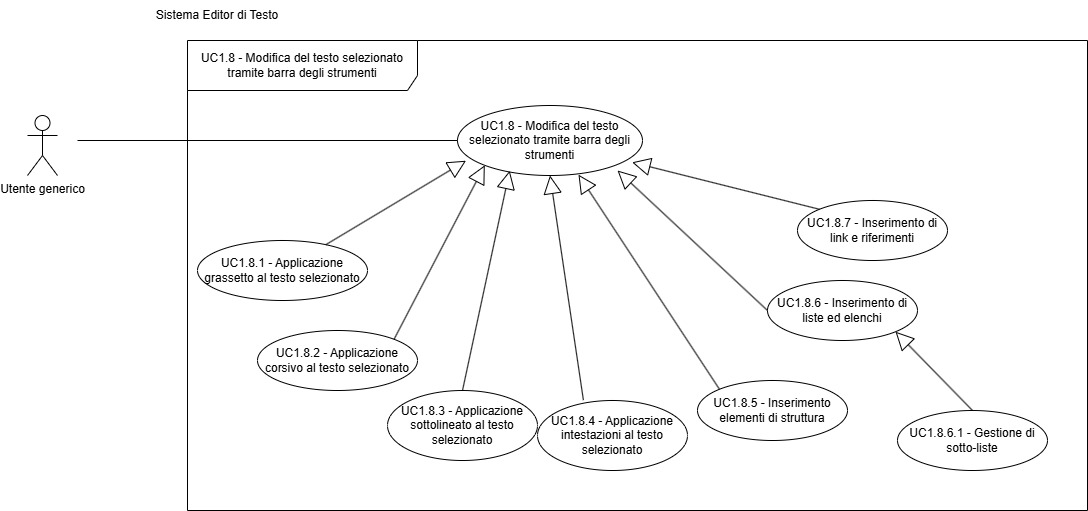
\includegraphics[width=0.8\textwidth]{../UCimg/UC1.8.jpg}
    \caption{Diagramma dei casi d'uso UC-1.8.*}
    \label{fig:uc1.8}
\end{figure}

\subsubsection{UC-1.9 - Impostare formattazioni senza testo presente nell'editor}
\begin{itemize}
    \item \textbf{Attore principale}: Utente generico
    \item \textbf{Descrizione}: Applicazione di formattazioni tramite barra degli strumenti senza che l'utente abbia già digitato del testo nell'editor
    \item \textbf{Precondizioni}: L’editor è aperto e l'utente ha accesso agli strumenti di formattazione
    \item \textbf{Postcondizioni}: Il testo futuro viene formattato in base alla formattazione già selezionata dall'utente prima della scrittura di testo 
    \item \textbf{Scenario principale}:
        \begin{itemize}
            \item L’utente seleziona la formattazione per il testo futuro
            \item Il sistema applica automaticamente la sintassi Markdown corrispondente
            \item Il testo scritto dall'utente prende automaticamente la formattazione applicata
        \end{itemize}
    \item \textbf{Estensioni}:
        \begin{itemize}
            \item Combinazione di più formattazioni diverse
        \end{itemize}
\end{itemize}

\subsubsection{UC-1.9.0.1 - Gestione multiple opzioni di formattazione}
\begin{itemize}
    \item \textbf{Attore principale}: Utente generico
    \item \textbf{Descrizione}: L'utente vuole scrivere del testo futuro con più formattazioni contemporaneamente
    \item \textbf{Precondizioni}: L’utente ha abilitiato diversi strumenti di formattazione
    \item \textbf{Postcondizioni}: Il testo futuro viene formattato con tutte le opzioni selezionate
    \item \textbf{Scenario principale}:
        \begin{itemize}
            \item L'utente applica più opzioni di formattazione per il testo futuro
            \item Il sistema applica tutte le formattazioni selezionate al testo futuro
            \item Il testo scritto dall'utente prende automaticamente tutte le formattazioni selezionate
            \item Il testo formattato viene visualizzato correttamente nell'anteprima
        \end{itemize}
\end{itemize}

\subsubsection{UC-1.9.1 - Impostare grassetto al testo futuro}
\begin{itemize}
    \item \textbf{Attore principale}: Utente generico
    \item \textbf{Descrizione}: Formattazione del testo futuro scritto dall’utente in grassetto
    \item \textbf{Precondizioni}: L’utente ha accesso alla formattazione in grassetto
    \item \textbf{Postcondizioni}: Il testo scritto è in grassetto
    \item \textbf{Scenario principale}:
        \begin{itemize}
            \item L’utente clicca sul pulsante "Grassetto" nella toolbar
            \item Il sistema applica la sintassi Markdown per il grassetto
            \item Il testo scritto successivamente dall'utente prende automaticamente la formattazione in grassetto
            \item Il testo in grassetto viene visualizzato correttamente nell'anteprima
        \end{itemize}
\end{itemize}

\subsubsection{UC-1.9.2 - Impostare corsivo al testo futuro}
\begin{itemize}
    \item \textbf{Attore principale}: Utente generico
    \item \textbf{Descrizione}: Formattazione del testo futuro scritto dall’utente in corsivo
    \item \textbf{Precondizioni}: L’utente ha accesso alla formattazione in corsivo
    \item \textbf{Postcondizioni}: Il testo scritto è in corsivo
    \item \textbf{Scenario principale}:
        \begin{itemize}
            \item L’utente clicca sul pulsante "Corsivo" nella toolbar
            \item Il sistema applica la sintassi Markdown per il corsivo
            \item Il testo scritto successivamente dall'utente prende automaticamente la formattazione in corsivo
            \item Il testo in corsivo viene visualizzato correttamente nell'anteprima
        \end{itemize}
\end{itemize}

\subsubsection{UC-1.9.3 - Impostare sottolineato al testo futuro}
\begin{itemize}
    \item \textbf{Attore principale}: Utente generico
    \item \textbf{Descrizione}: Formattazione del testo futuro scritto dall’utente in modalità sottolineata

    \item \textbf{Precondizioni}: L’utente ha accesso alla formattazione sottolineata
    \item \textbf{Postcondizioni}: Il testo scritto è sottolineato
    \item \textbf{Scenario principale}:
        \begin{itemize}
            \item L’utente clicca sul pulsante "Sottolineato" nella toolbar
            \item Il sistema applica la sintassi Markdown per la sottolineatura
            \item Il testo scritto successivamente dall'utente prende automaticamente la sottolineatura
            \item Il testo sottolineato viene visualizzato correttamente nell'anteprima
        \end{itemize}
\end{itemize}

\subsubsection{UC-1.9.4 - Impostare intestazioni}
\begin{itemize}
    \item \textbf{Attore principale}: Utente generico
    \item \textbf{Descrizione}: Formattazione del testo futuro scritto dall’utente rispettando le intestazioni
    \item \textbf{Precondizioni}: L’utente ha accesso alla formattazione per le intestazioni
    \item \textbf{Postcondizioni}: Il testo scritto presenta le intestazioni
    \item \textbf{Scenario principale}:
        \begin{itemize}
            \item L’utente clicca sul pulsante "Intestazioni" nella toolbar
            \item L’utente applica un’intestazione tramite:
                \begin{enumerate}
                    \item Toolbar (H1, H2, H3, ecc.)
                    \item Sintassi Markdown (\#, \#\#, \#\#\#)
                \end{enumerate}
            \item Il testo scritto successivamente dall'utente prende automaticamente la formattazione dell'intestazione
            \item L'intestazione viene visualizzata correttamente nell'anteprima
        \end{itemize}
\end{itemize}

\subsubsection{UC-1.9.5 - Impostare struttura al documento}
\begin{itemize}
    \item \textbf{Attore principale}: Utente generico
    \item \textbf{Descrizione}: Formattazione del testo futuro scritto dall’utente secondo una struttura da lui selezionata
    \item \textbf{Precondizioni}: L’utente ha accesso alla formattazione per la gestione della struttura
    \item \textbf{Postcondizioni}: Il testo scritto rispetta la struttura selezionata dall’utente
    \item \textbf{Scenario principale}:
        \begin{itemize}
            \item L’utente clicca sul pulsante "Struttura" nella toolbar
            \item L’utente sceglie il tipo di struttura da applicare:
                \begin{enumerate}
                    \item Tabella
                    \item Separatore orizzontale
                \end{enumerate}
            \item L'elemento viene visualizzato correttamente nell'anteprima
        \end{itemize}
\end{itemize}

\subsubsection{UC-1.9.6 - Impostare liste ed elenchi}
\begin{itemize}
    \item \textbf{Attore principale}: Utente generico
    \item \textbf{Descrizione}: Formattazione del testo futuro scritto dall’utente secondo una lista o un elenco
    \item \textbf{Precondizioni}: L’utente ha accesso alla formattazione per la gestione delle liste ed elenchi
    \item \textbf{Postcondizioni}: Il testo scritto è in formato lista/elenco
    \item \textbf{Scenario principale}:
        \begin{itemize}
            \item L’utente clicca sul pulsante "Liste ed elenchi" nella toolbar
            \item L’utente sceglie il tipo di elenco da applicare:
                \begin{itemize}
                    \item ordinato/non ordinato
                \end{itemize}
            \item La formattazione viene applicata e l'utente può inserire testo nella lista già pronta
            \item La lista viene visualizzata correttamente nell'anteprima
        \end{itemize}
\end{itemize}

\subsubsection{UC-1.9.7 - Impostare link e riferimenti}
\begin{itemize}
    \item \textbf{Attore principale}: Utente generico
    \item \textbf{Descrizione}: Formattazione per l’inserimento dei link o riferimenti
    \item \textbf{Precondizioni}:L’utente ha accesso alla formattazione per la gestione dei link e riferimenti
    \item \textbf{Postcondizioni}:Il testo scritto è un link/riferimento
    \item \textbf{Scenario principale}:
        \begin{itemize}
            \item L’utente clicca sul comando ”Inserisci link o riferimento”
            \item L’utente inserisce l’URL di destinazione
            \item Il sistema applica la sintassi Markdown per il link o riferimenti
            \item Il link viene visualizzato correttamente nell'anteprima
        \end{itemize}
\end{itemize}

\begin{figure}[H]
    \centering
    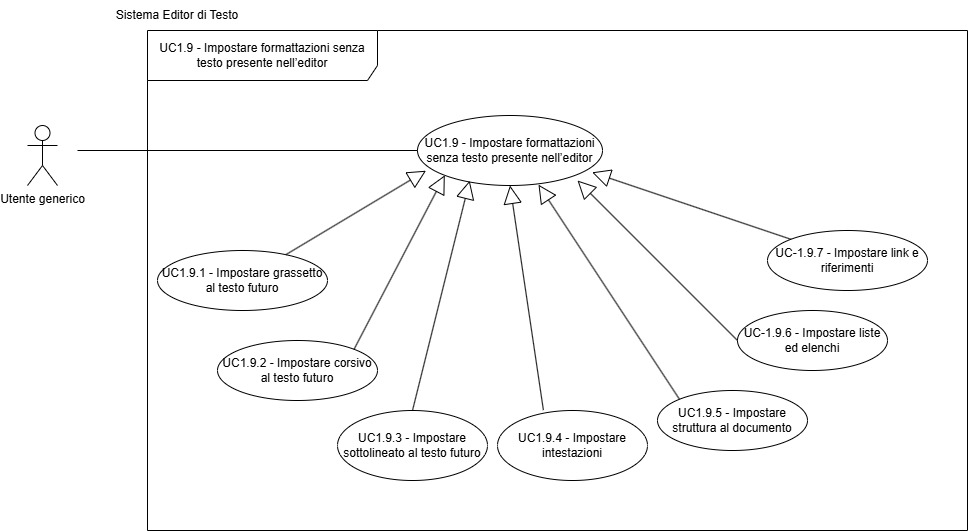
\includegraphics[width=0.8\textwidth]{../UCimg/UC1.9.jpg}
    \caption{Diagramma dei casi d'uso UC-1.9.*}
    \label{fig:uc1.9}
\end{figure}

\subsubsection{UC-1.10 - Gestione modalità di visualizzazione}
\begin{itemize}
    \item \textbf{Attore principale}: Utente generico
    \item \textbf{Descrizione}: Selezione della modalità di visualizzazione dell’area di lavoro per alternare tra scrittura, anteprima o visione combinata
    \item \textbf{Precondizioni}: L’editor è aperto e funzionante
    \item \textbf{Postcondizioni}: L’interfaccia viene adattata alla modalità di visualizzazione selezionata
    \item \textbf{Scenario principale}:
        \begin{itemize}
            \item L’utente accede ai comandi di visualizzazione
            \item ’utente seleziona la modalità di visualizzazione desiderata tra quelle disponibili
            \item Il sistema riconfigura i pannelli dell'interfaccia in base alla scelta effettuata
        \end{itemize}
\end{itemize}

\subsubsection{UC-1.10.1 - Modalità di visualizzazione solo editor}
\begin{itemize}
    \item \textbf{Attore principale}: Utente generico
    \item \textbf{Descrizione}: Cambia la modalità di visualizzazione dell’editor, che mostra solo l'area di scrittura dell'editor
    \item \textbf{Precondizioni}: La modalità di visualizzazione comprende solo il documento formattato oppure è in modalità split view
    \item \textbf{Postcondizioni}: Visualizzazione esclusiva dell'area di testo dell'editor
    \item \textbf{Scenario principale}:
        \begin{itemize}
            \item L'utente seleziona la modalità di visualizzazione "Solo editor" (sintassi Markdown visibile)
            \item Il sistema adatta l'interfaccia alla modalità scelta
        \end{itemize}
\end{itemize}


\subsubsection{UC-1.10.2 - Modalità di visualizzazione solo documento formattato}
\begin{itemize}
    \item \textbf{Attore principale}: Utente generico
    \item \textbf{Descrizione}: Cambia la modalità di visualizzazione dell'editor, che mostra solo l'anteprima formattata del documento
    \item \textbf{Precondizioni}: La modalità di visualizzazione comprende solo l’editor oppure è in modalità split view
    \item \textbf{Postcondizioni}: Visualizzazione esclusiva del documento formattato
    \item \textbf{Scenario principale}:
        \begin{itemize}
            \item L'utente seleziona la modalità di visualizzazione "Solo documento"/"Solo anteprima"
            \item Il sistema adatta l'interfaccia alla modalità scelta
        \end{itemize}
\end{itemize}

\subsubsection{UC-1.10.3 - Modalità di visualizzazione split view}
\begin{itemize}
    \item \textbf{Attore principale}: Utente generico
    \item \textbf{Descrizione}: Cambia la modalità di visualizzazione in split view, che mostra sia l'area di testo sia l'anteprima del documento formattato
    \item \textbf{Precondizioni}: La modalità di visualizzazione comprende solo l’editor oppure solo il documento
    \item \textbf{Postcondizioni}: Visualizzazione split view dell’area di testo e del documento formattato
    \item \textbf{Scenario principale}:
        \begin{itemize}
            \item L'utente seleziona la modalità di visualizzazione "Split View"
            \item Il sistema adatta l'interfaccia alla modalità scelta
        \end{itemize}
\end{itemize}

\begin{figure}[H]
    \centering
    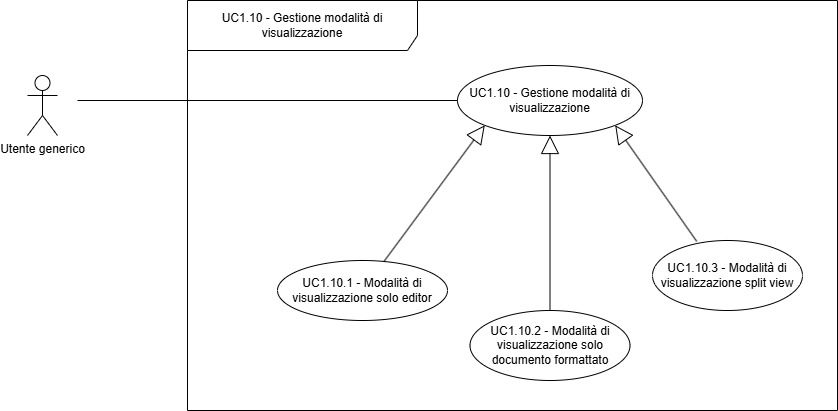
\includegraphics[width=0.8\textwidth]{../UCimg/UC1.10.jpg}
    \caption{Diagramma dei casi d'uso UC-1.10, 1.10.*}
    \label{fig:uc1.10}
\end{figure}

\subsubsection{UC-1.11 - Ricerca nel testo}
\begin{itemize}
    \item \textbf{Attore principale}: Utente generico
    \item \textbf{Descrizione}: Ricerca di occorrenze di testo all'interno del documento
    \item \textbf{Precondizioni}: È presente testo nell'editor
    \item \textbf{Postcondizioni}: Vengono trovate occorrenze di testo
    \item \textbf{Scenario principale}:
        \begin{itemize}
            \item L'utente attiva la funzione "Ricerca"
            \item L'utente inserisce il testo da cercare
            \item Il sistema evidenzia le occorrenze trovate
        \end{itemize}
    \item \textbf{Estensioni}:
        \begin{itemize}
            \item Nessuna occorrenza trovata
        \end{itemize}
\end{itemize}

\subsubsection{UC-1.11.1 - Gestione assenza di occorrenze}
\begin{itemize}
    \item \textbf{Attore principale}: Utente generico
    \item \textbf{Descrizione}: La ricerca non trova occorrenze di testo nell'editor
    \item \textbf{Precondizioni}: L'utente effettua una ricerca
    \item \textbf{Postcondizioni}: L'utente viene informato che nessuna occorrenza è stata trovata
    \item \textbf{Scenario}:
        \begin{itemize}
            \item L'utente attiva la funzione "Ricerca"
            \item L'utente inserisce il testo da cercare
            \item Il sistema non trova occorrenze
            \item Il sistema informa l'utente che nessuna occorrenza è stata trovata con un messaggio
        \end{itemize}
\end{itemize}

\begin{figure}[H]
    \centering
    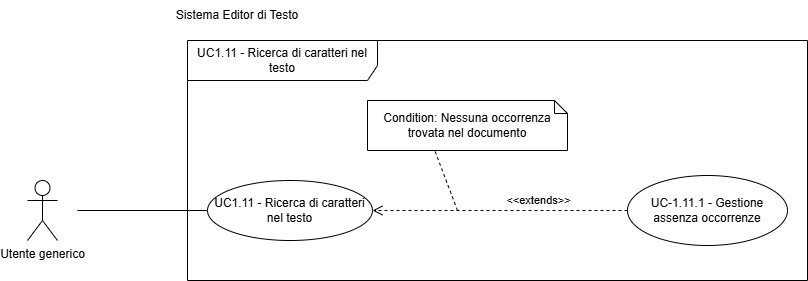
\includegraphics[width=0.8\textwidth]{../UCimg/UC1.11.jpg}
    \caption{Diagramma dei casi d'uso UC-1.11, 1.11.1}
    \label{fig:uc1.11}
\end{figure}

\newpage

\subsection{Macroarea 2 - Funzionalità AI}
\subsubsection{UC-2.0 - Distinzione del Testo Utente da quello Generato}
\begin{itemize}
    \item \textbf{Attore principale}: Utente generico
    \item \textbf{Descrizione}: Sistema di formattazione che rende chiaramente distinguibile il testo generato dall’AI dal testo scritto dall’utente
    \item \textbf{Precondizioni}: Nell’editor è presente sia testo digitato dall’utente che testo generato dall’AI
    \item \textbf{Postcondizioni}: Il testo generato è chiaramente distinguibile dal testo dell’utente
    \item \textbf{Scenario principale}:
        \begin{itemize}
            \item L’utente seleziona un’operazione AI
            \item L’editor inserisce il testo generato all’interno del documento
            \item Il sistema formatta automaticamente il testo generato con elementi di stile che lo rendono diverso dal testo scritto dall’utente
            \item Il sistema inserisce automaticamente degli elementi di separazione tra il testo generato e il testo originale dell’utente
        \end{itemize}
\end{itemize}

\subsubsection{UC-2.1 - Interazione con i testi Generati dall’AI}
\begin{itemize}
    \item \textbf{Attore principale}: Utente generico
    \item \textbf{Descrizione}: Gestione della storia e interazione con tutti i testi generati dall’AI all’interno del documento
    \item \textbf{Precondizioni}: Sono state eseguite una o più operazioni AI e i relativi testi generati sono stati inseriti nell’editor
    \item \textbf{Postcondizioni}: L’utente può visualizzare e operare sull’intera sequenza di generazioni AI accumulate nel documento
    \item \textbf{Scenario principale}:
    \begin{itemize}
        \item L’utente seleziona un’operazione AI da eseguire nel testo selezionato o non selezionato
        \item Ogni nuova operazione AI genera testo che viene inserito nell’editor in una sezione apposita
        \item Queste sezioni sono considerate delle proposte, che includono le seguenti opzioni: accetta, annulla, rigenera
        \item Ogni blocco mantiene la sua formattazione distintiva che identifica:
            \begin{enumerate}
                \item Il tipo di operazione
                \item La data/ora di generazione
                \item I parametri specifici (lingua, cappello, ecc.)
            \end{enumerate}
    \end{itemize}
    \item \textbf{Estensioni}:
    \begin{itemize}
        \item L’utente può modificare o effettuare operazioni sulle generazioni
        \item L’utente può confermare, eliminare o rigenerare la risposta dell’AI
        \item L’utente vuole una vista compatta della storia delle generazioni
        \item L’utente vuole vedere solo il testo digitato senza i blocchi di testo generati dall’AI
        \item L’utente annulla l’operazione prima del completamento della generazione
        \item Il servizio LLM restituisce un errore senza dare risposta
    \end{itemize}
\end{itemize}

\begin{figure}[H]
    \centering
    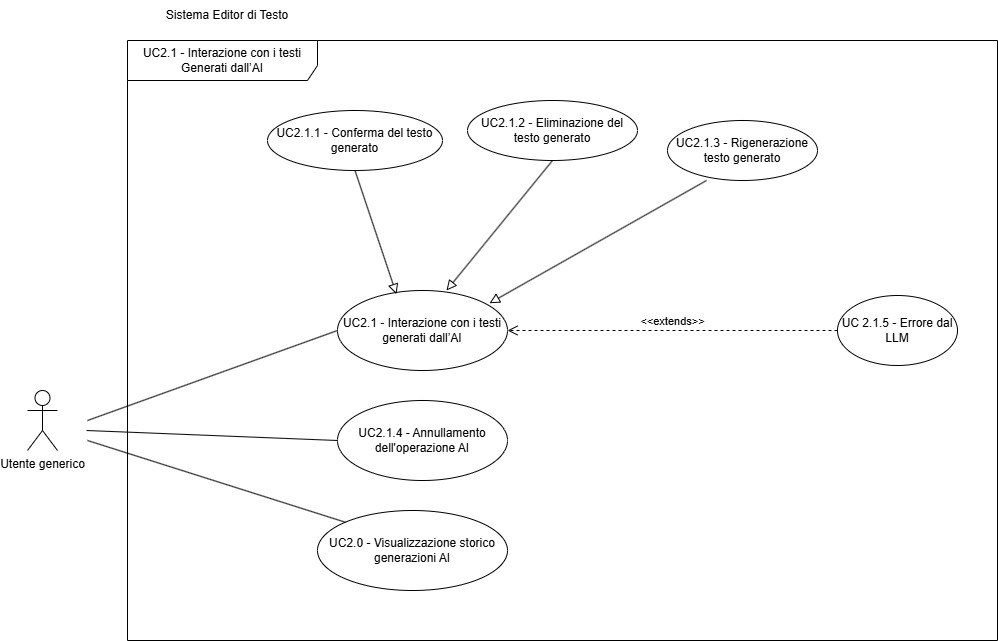
\includegraphics[width=0.8\textwidth]{../UCimg/UC2.1.jpg}
    \caption{Diagramma dei casi d'uso UC-2.1, 2.1.*}
    \label{fig:uc2.1}
\end{figure}

\subsubsection{UC-2.1.1 - Conferma del testo generato}
\begin{itemize}
    \item \textbf{Attore principale}: Utente generico
    \item \textbf{Descrizione}: L’utente decide di accettare la proposta di testo generata dall'AI
    \item \textbf{Precondizioni}: Il foglio di lavoro contiene una proposta di testo, generata dall’AI
    \item \textbf{Postcondizioni}: L’utente accetta la proposta di testo e viene integrata nel documento
    \item \textbf{Scenario principale}:
    \begin{itemize}
        \item L’utente visualizza una proposta di testo generata dall’AI
        \item L’utente seleziona l’opzione "Accetta"
        \item Il testo generato viene integrato nel documento
    \end{itemize}
\end{itemize}

\subsubsection{UC-2.1.2 - Modifica del testo generato}
\begin{itemize}
    \item \textbf{Attore principale}: Utente generico
    \item \textbf{Descrizione}: L’utente può interagire con il testo generato dall’AI modificandolo tramite sintassi markdown
    \item \textbf{Precondizioni}: Sono state eseguite una o più operazioni AI e i relativi testi generati sono stati inseriti nell’editor
    \item \textbf{Postcondizioni}: L’utente modifica i testi generati dall’AI accumulati nel file
    \item \textbf{Scenario principale}:
    \begin{itemize}
        \item L’utente individua un blocco di testo generato dall’AI
        \item L’utente seleziona tutto o una parte del testo generato
        \item L’utente applica una formattazione markdown al testo selezionato
    \end{itemize}
\end{itemize}

\subsubsection{UC-2.1.3 - Eliminazione del testo generato}
\begin{itemize}
    \item \textbf{Attore principale}: Utente generico
    \item \textbf{Descrizione}: L’utente può eliminare intere sezioni di testo generato dall’AI
    \item \textbf{Precondizioni}: Sono state eseguite una o più operazioni AI e i relativi testi generati sono stati inseriti nell’editor
    \item \textbf{Postcondizioni}: L’utente elimina il testo generato
    \item \textbf{Scenario principale}:
    \begin{itemize}
        \item L’utente individua un blocco di testo generato dall’AI
        \item L’utente visualizza l’opzione "Annulla" accanto alla generazione
        \item L’utente seleziona “Annulla”
        \item Il testo generato viene cancellato dal documento
    \end{itemize}
\end{itemize}

\subsubsection{UC-2.1.4 - Rigenerazione testo generato}
\begin{itemize}
    \item \textbf{Attore principale}: Utente generico
    \item \textbf{Descrizione}: L’utente può rigenerare intere sezioni di testo precedentemente generato dall’AI
    \item \textbf{Precondizioni}: Sono state eseguite una o più operazioni AI e i relativi testi generati sono stati inseriti nell’editor
    \item \textbf{Postcondizioni}: Il testo generato precedentemente viene sostituito da una nuova variante prodotta dall'AI
    \item \textbf{Scenario principale}:
    \begin{itemize}
        \item L’utente individua un blocco di testo generato dall’AI
        \item L’utente visualizza l’opzione “Rigenera” accanto alla generazione
        \item L’utente seleziona “Rigenera”
        \item Il sistema invia nuovamente la richiesta all'AI utilizzando gli stessi parametri
        \item Il testo precedentemente generato viene sovrascritto da una nuova generazione
    \end{itemize}
\end{itemize}

\subsubsection{UC-2.1.5 - Visualizzazione del registro delle generazioni}
\begin{itemize}
    \item \textbf{Attore principale}: Utente generico
    \item \textbf{Descrizione}: L'utente può scegliere di visualizzare solo il testo che è stato generato dalle funzionalità AI, consultando un registro delle generazioni
    \item \textbf{Precondizioni}: Sono state eseguite una o più operazioni AI e i relativi testi generati vengono in contemporanea inseriti in un registro dedicato
    \item \textbf{Postcondizioni}: L'utente visualizza il registro delle generazioni
    \item \textbf{Scenario principale}:
    \begin{itemize}
        \item L’utente seleziona l’opzione “Visualizza storico generazioni”
        \item Il sistema mostra un registro con tutte le generazioni AI effettuate nel documento
    \end{itemize}
\end{itemize}

\subsubsection{UC-2.1.6 - Annullamento dell’operazione}
\begin{itemize}
    \item \textbf{Attore principale}: Utente generico
    \item \textbf{Descrizione}: L’utente interrompe volontariamente una richiesta AI in corso prima del suo completamento
    \item \textbf{Precondizioni}: L'utente ha avviato un'operazione AI e il sistema è in fase di elaborazione
    \item \textbf{Postcondizioni}: L’operazione viene annullata e il documento rimane nello stato precedente alla richiesta
    \item \textbf{Scenario principale}:
    \begin{itemize}
        \item Il sistema sta elaborando una richiesta AI
        \item L’editor mostra un indicatore di attesa (opzionale)
        \item L’utente seleziona l’opzione “Annulla” per l’operazione in corso
        \item L’editor interrompe l’operazione e la comunicazione con il servizio LLM
        \item Il testo presente nell’editor rimane invariato
    \end{itemize}
\end{itemize}

\subsubsection{UC-2.1.7 - Errore dal LLM}
\begin{itemize}
    \item \textbf{Attore principale}: Utente generico
    \item \textbf{Descrizione}: Il sistema gestisce un fallimento nella generazione della risposta da parte del LLM (es. timeout, assenza di connessione, errore server)
    \item \textbf{Precondizioni}: L'utente ha avviato un'operazione AI e il sistema è in fase di elaborazione
    \item \textbf{Postcondizioni}: L’utente viene informato dell'errore e il documento rimane nello stato precedente alla richiesta
    \item \textbf{Scenario principale}:
    \begin{itemize}
        \item Il sistema tenta di comunicare con il servizio LLM esterno
        \item Il servizio LLM non risponde o restituisce un codice di errore
        \item Il sistema intercetta l'errore interrompendo il processo di attesa
        \item L’editor manda un messaggio di errore
        \item Il testo presente nell’editor rimane invariato
    \end{itemize}
\end{itemize}

\subsubsection{UC-2.2 - Riassunto del testo}
\begin{itemize}
    \item \textbf{Attore principale}: Utente generico
    \item \textbf{Descrizione}: Generazione di un riassunto del testo selezionato o dell’intero documento
    \item \textbf{Precondizioni}: L’editor contiene del testo
    \item \textbf{Postcondizioni}: Un nuovo blocco di testo contenente il riassunto viene inserito nell’editor, formattato in modo distinto rispetto al testo originale
    \item \textbf{Scenario principale}:
    \begin{itemize}
        \item L’utente seleziona una porzione di testo (o non seleziona nulla per indicare l'intero documento)
        \item L’utente attiva il comando ”Riassumi”
        \item Il sistema elabora la richiesta e invia il testo al LLM
        \item Il sistema genera il riassunto e lo inserisce nell'editor, dopo il testo originale selezionato, applicando lo stile distintivo per il testo generato
    \end{itemize}
\end{itemize}

\begin{figure}[H]
    \centering
    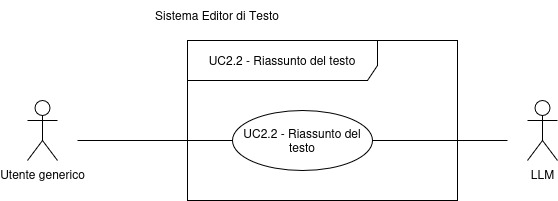
\includegraphics[width=0.8\textwidth]{../UCimg/UC2.2.jpg}
    \caption{Diagramma dei casi d'uso UC-2.2}
    \label{fig:uc2.2}
\end{figure}

\subsubsection{UC-2.3 - Riscrittura del testo}
\begin{itemize}
    \item \textbf{Attore principale}: Utente generico
    \item \textbf{Descrizione}: Rielaborazione del testo per modificarne stile, sintassi e chiarezza
    \item \textbf{Precondizioni}: L’editor contiene del testo
    \item \textbf{Postcondizioni}: Una variante riscritta del testo viene inserita nell’editor con formattazione distintiva, preservando il testo originale
    \item \textbf{Scenario principale}:
    \begin{itemize}
        \item L’utente seleziona il testo da riscrivere
        \item L’utente attiva il comando ”Riscrivi”
        \item L’utente specifica come riscrivere il testo (opzionale)
        \item Il sistema elabora la richiesta e invia il testo al LLM
        \item Il sistema riscrive il testo e lo inserisce nell'editor, dopo il testo originale selezionato, applicando lo stile distintivo per il testo generato
    \end{itemize}
\end{itemize}

\begin{figure}[H]
    \centering
    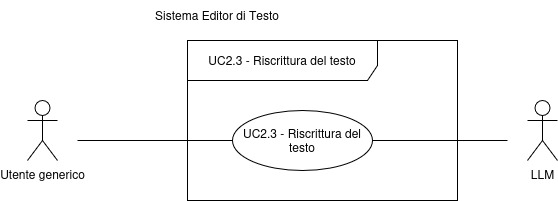
\includegraphics[width=0.8\textwidth]{../UCimg/UC2.3.jpg}
    \caption{Diagramma dei casi d'uso UC-2.3}
    \label{fig:uc2.3}
\end{figure}

\subsubsection{UC-2.4 - Traduzione del testo}
\begin{itemize}
    \item \textbf{Attore principale}: Utente generico
    \item \textbf{Descrizione}: Traduzione automatica del testo nella lingua selezionata
    \item \textbf{Precondizioni}: È presente testo nell’editor (completo o selezionato)
    \item \textbf{Postcondizioni}: La traduzione viene generata e inserita nel documento con la formattazione distintiva del testo AI
    \item \textbf{Scenario principale}:
    \begin{itemize}
        \item L’utente seleziona la porzione di testo da tradurre (o nessuna selezione per l'intero documento)
        \item L’utente attiva il comando ”Traduci”
        \item L’utente definisce la lingua di destinazione
        \item Il sistema elabora la richiesta e invia il testo al LLM
        \item Il sistema mostra la traduzione generata
        \item Il sistema inserisce il testo nell'editor, dopo il testo originale selezionato, applicando lo stile distintivo per il testo generato
    \end{itemize}
    \item \textbf{Estensioni}:
    \begin{itemize}
        \item Il testo è già nella lingua selezionata: il testo originale rimane invariato e il sistema manda un messaggio all’utente
        \item L’utente non seleziona nessuna lingua di destinazione
    \end{itemize}
\end{itemize}

\subsubsection{UC-2.4.1 - Gestione mancata selezione della lingua di destinazione}
\begin{itemize}
    \item \textbf{Attore principale}: Utente generico
    \item \textbf{Descrizione}: L’utente attiva l’operazione di traduzione senza aver confermato una lingua di destinazione
    \item \textbf{Precondizioni}: È presente testo nell’editor (completo o selezionato) e l’utente attiva il comando di traduzione
    \item \textbf{Postcondizioni}: Viene generata la traduzione in inglese e viene inserita nel documento con la formattazione distintiva del testo AI
    \item \textbf{Scenario principale}:
    \begin{itemize}
        \item L’utente seleziona la porzione di testo da tradurre (o nessuna selezione per l'intero documento)
        \item L’utente attiva il comando ”Traduci” senza selezionare una lingua di destinazione
        \item Il sistema imposta la lingua inglese come lingua di default per la traduzione
        \item Il sistema elabora la richiesta e invia il testo al LLM
        \item Il sistema mostra la traduzione generata
        \item Il sistema inserisce il testo nell'editor, dopo il testo originale selezionato, applicando lo stile distintivo per il testo generato
    \end{itemize}
\end{itemize}

\begin{figure}[H]
    \centering
    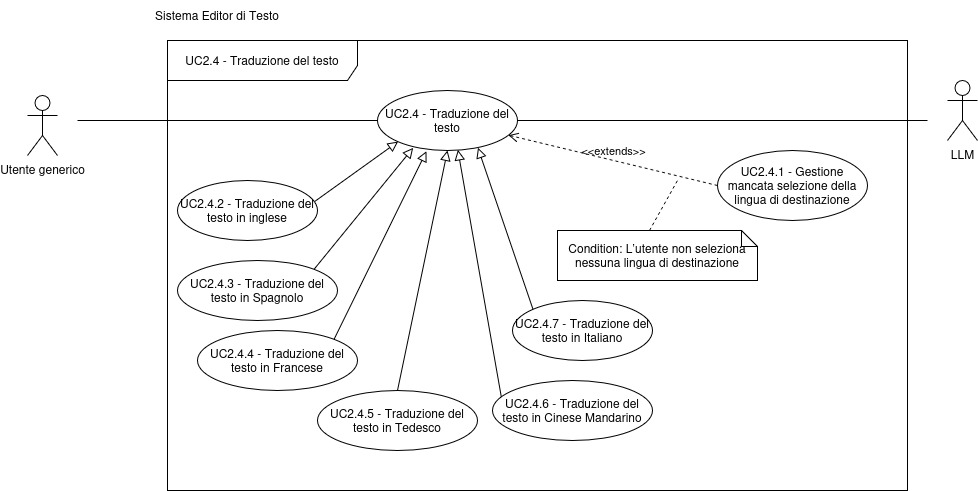
\includegraphics[width=0.8\textwidth]{../UCimg/UC2.4.jpg}
    \caption{Diagramma dei casi d'uso UC-2.4.*}
    \label{fig:uc2.4}
\end{figure}

\subsubsection{UC-2.4.2 - Traduzione del testo in inglese}
\begin{itemize}
    \item \textbf{Attore principale}: Utente generico
    \item \textbf{Descrizione}: Traduzione automatica del testo nella lingua inglese
    \item \textbf{Precondizioni}: È presente testo nell’editor (completo o selezionato)
    \item \textbf{Postcondizioni}: Il testo viene tradotto in lingua inglese e inserito nel documento con la formattazione distintiva del testo AI
    \item \textbf{Scenario principale}:
    \begin{itemize}
        \item L’utente seleziona la porzione di testo da tradurre (o nessuna selezione per l'intero documento)
        \item L’utente attiva il comando ”Traduci”
        \item L’utente imposta “Inglese” come lingua di destinazione
        \item Il sistema elabora la richiesta e invia il testo al LLM
        \item Il sistema mostra la traduzione generata
        \item Il sistema inserisce il testo nell'editor, dopo il testo originale selezionato, applicando lo stile distintivo per il testo generato
    \end{itemize}
\end{itemize}

\subsubsection{UC-2.4.3 - Traduzione del testo in Spagnolo}
\begin{itemize}
    \item \textbf{Attore principale}: Utente generico
    \item \textbf{Descrizione}: Traduzione automatica del testo nella lingua spagnola
    \item \textbf{Precondizioni}: È presente testo nell’editor (completo o selezionato)
    \item \textbf{Postcondizioni}: Il testo viene tradotto in lingua spagnola e inserito nel documento con la formattazione distintiva del testo AI
    \item \textbf{Scenario principale}:
    \begin{itemize}
        \item L’utente seleziona la porzione di testo da tradurre (o nessuna selezione per l'intero documento)
        \item L’utente attiva il comando ”Traduci”
        \item L’utente imposta “Spagnolo” come lingua di destinazione
        \item Il sistema elabora la richiesta e invia il testo al LLM
        \item Il sistema mostra la traduzione generata
        \item Il sistema inserisce il testo nell'editor, dopo il testo originale selezionato, applicando lo stile distintivo per il testo generato
    \end{itemize}
\end{itemize}

\subsubsection{UC-2.4.4 - Traduzione del testo in Francese}
    \begin{itemize}
    \item \textbf{Attore principale}: Utente generico
    \item \textbf{Descrizione}: Traduzione automatica del testo nella lingua francese
    \item \textbf{Precondizioni}: È presente testo nell’editor (completo o selezionato)
    \item \textbf{Postcondizioni}: Il testo viene tradotto in lingua francese e inserito nel documento con la formattazione distintiva del testo AI
    \item \textbf{Scenario principale}:
    \begin{itemize}
        \item L’utente seleziona la porzione di testo da tradurre (o nessuna selezione per l'intero documento)
        \item L’utente attiva il comando ”Traduci”
        \item L’utente imposta “Francese” come lingua di destinazione
        \item Il sistema elabora la richiesta e invia il testo al LLM
        \item Il sistema mostra la traduzione generata
        \item Il sistema inserisce il testo nell'editor, dopo il testo originale selezionato, applicando lo stile distintivo per il testo generato
    \end{itemize}
\end{itemize}

\subsubsection{UC-2.4.5 - Traduzione del testo in Tedesco}
\begin{itemize}
    \item \textbf{Attore principale}: Utente generico
    \item \textbf{Descrizione}: Traduzione automatica del testo nella lingua tedesca
    \item \textbf{Precondizioni}: È presente testo nell’editor (completo o selezionato)
    \item \textbf{Postcondizioni}: Il testo viene tradotto in lingua tedesca e inserito nel documento con la formattazione distintiva del testo AI
    \item \textbf{Scenario principale}:
    \begin{itemize}
        \item L’utente seleziona la porzione di testo da tradurre (o nessuna selezione per l'intero documento)
        \item L’utente attiva il comando ”Traduci”
        \item L’utente imposta “Tedesco” come lingua di destinazione
        \item Il sistema elabora la richiesta e invia il testo al LLM
        \item Il sistema mostra la traduzione generata
        \item Il sistema inserisce il testo nell'editor, dopo il testo originale selezionato, applicando lo stile distintivo per il testo generato
    \end{itemize}
\end{itemize}

\subsubsection{UC-2.4.6 - Traduzione del testo in Cinese Mandarino}
\begin{itemize}
    \item \textbf{Attore principale}: Utente generico
    \item \textbf{Descrizione}: Traduzione automatica del testo nella lingua cinese mandarino
    \item \textbf{Precondizioni}: È presente testo nell’editor (completo o selezionato)
    \item \textbf{Postcondizioni}: Il testo viene tradotto in lingua cinese mandarino e inserito nel documento con la formattazione distintiva del testo AI
    \item \textbf{Scenario principale}:
    \begin{itemize}
        \item L’utente seleziona la porzione di testo da tradurre (o nessuna selezione per l'intero documento)
        \item L’utente attiva il comando ”Traduci”
        \item L’utente imposta “Cinese Mandarino” come lingua di destinazione
        \item Il sistema elabora la richiesta e invia il testo al LLM
        \item Il sistema mostra la traduzione generata
        \item Il sistema inserisce il testo nell'editor, dopo il testo originale selezionato, applicando lo stile distintivo per il testo generato
    \end{itemize}
\end{itemize}

\subsubsection{UC-2.4.7 - Traduzione del testo in Italiano}
\begin{itemize}
    \item \textbf{Attore principale}: Utente generico
    \item \textbf{Descrizione}: Traduzione automatica del testo nella lingua Italiana
    \item \textbf{Precondizioni}: È presente testo nell’editor (completo o selezionato)
    \item \textbf{Postcondizioni}: Il testo viene tradotto in lingua Italiana e inserito nel documento con la formattazione distintiva del testo AI
    \item \textbf{Scenario principale}:
    \begin{itemize}
        \item L’utente seleziona la porzione di testo da tradurre (o nessuna selezione per l'intero documento)
        \item L’utente attiva il comando ”Traduci”
        \item L’utente imposta “Italiano” come lingua di destinazione
        \item Il sistema elabora la richiesta e invia il testo al LLM
        \item Il sistema mostra la traduzione generata
        \item Il sistema inserisce il testo nell'editor, dopo il testo originale selezionato, applicando lo stile distintivo per il testo generato
    \end{itemize}
\end{itemize}

\subsubsection{UC-2.5 - Correzione grammaticale}
\begin{itemize}
    \item \textbf{Attore principale}: Utente generico
    \item \textbf{Descrizione}: Rilevamento e correzione automatica di errori grammaticali, ortografici e di punteggiatura
    \item \textbf{Precondizioni}: È presente testo nell’editor (completo o selezionato)
    \item \textbf{Postcondizioni}: Una versione corretta del testo viene inserita nell’editor con formattazione distintiva, preservando il testo originale
    \item \textbf{Scenario principale}:
    \begin{itemize}
        \item L’utente seleziona la porzione di testo da correggere (o nessuna selezione per l'intero documento)
        \item L’utente attiva il comando ”Correggi”
        \item Il sistema elabora la richiesta e invia il testo al LLM
        \item Il sistema riscrive il testo corretto e lo inserisce nell'editor, dopo il testo originale selezionato, applicando lo stile distintivo per il testo generato
    \end{itemize}
    \item \textbf{Estensioni}:
    \begin{itemize}
        \item Non vengono rilevati errori
    \end{itemize}
\end{itemize}

\subsubsection{UC-2.5.1 - Nessun errore grammaticale rilevato}
\begin{itemize}
    \item \textbf{Attore principale}: Utente generico
    \item \textbf{Descrizione}: Dopo l’operazione di correzione grammaticale non vengono rilevati errori
    \item \textbf{Precondizioni}: È presente testo nell’editor (completo o selezionato) e l’utente ha attivato il comando di correzione grammaticale
    \item \textbf{Postcondizioni}: Non ci sono errori e il documento rimane invariato
    \item \textbf{Scenario principale}:
    \begin{itemize}
        \item Il sistema analizza il testo e non rileva errori
        \item Il sistema mostra una notifica all’utente
        \item Il testo originale rimane invariato e nessun nuovo blocco viene generato
    \end{itemize}
\end{itemize}

\begin{figure}[H]
    \centering
    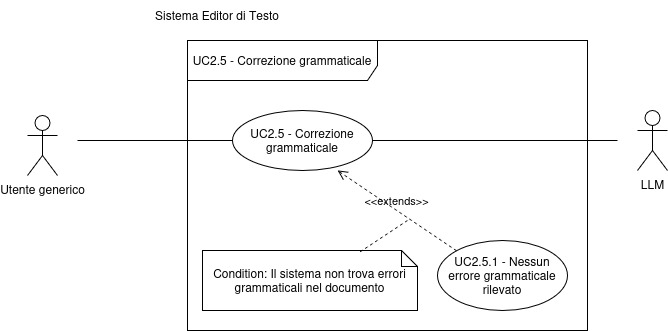
\includegraphics[width=0.8\textwidth]{../UCimg/UC2.5.jpg}
    \caption{Diagramma dei casi d'uso UC-2.5, 2.5.1}
    \label{fig:uc2.5}
\end{figure}

\subsubsection{UC-2.6 - Critica testuale con i 6 Cappelli di De Bono}
\begin{itemize}
    \item \textbf{Attore principale}: Utente generico
    \item \textbf{Descrizione}: Analisi del testo basata su una delle modalità del modello dei "Sei Cappelli per pensare" di Edward De Bono
    \item \textbf{Precondizioni}: È presente testo nell’editor (completo o selezionato)
    \item \textbf{Postcondizioni}: Viene generata un’analisi del testo secondo la prospettiva scelta e inserita nel documento con formattazione distintiva
    \item \textbf{Scenario principale}:
    \begin{itemize}
        \item L’utente seleziona la porzione di testo da analizzare (o nessuna selezione per l'intero documento)
        \item L’utente attiva il menu ”Analisi critica”
        \item L’utente definisce la modalità di analisi (colore del Cappello) desiderata
        \item Il sistema elabora la richiesta e invia il testo al LLM
        \item Il sistema genera l'analisi e la inserisce nell'editor, dopo il testo originale selezionato, applicando lo stile distintivo per il testo generato
    \end{itemize}
    \item \textbf{Estensioni}:
    \begin{itemize}
        \item Il testo è troppo breve per un’analisi significativa
        \item L’utente non seleziona nessun colore per l’analisi
    \end{itemize}
\end{itemize}

\subsubsection{UC-2.6.1 - Gestione testo insufficiente per analisi critica}
\begin{itemize}
    \item \textbf{Attore principale}: Utente generico
    \item \textbf{Descrizione}: Gestione dell’errore nel caso in cui il contenuto selezionato non sia sufficiente per applicare il modello di analisi dei Sei Cappelli
    \item \textbf{Precondizioni}: È presente testo nell’editor e l’utente attiva il comando di analisi su una porzione di testo
    \item \textbf{Postcondizioni}: L’operazione viene annullata e viene mostrato un messaggio di avviso. Il testo originale rimane invariato
    \item \textbf{Scenario principale}:
    \begin{itemize}
        \item L’utente seleziona una porzione di testo molto breve da analizzare (o il documento contiene testo insufficiente)
        \item L’utente attiva il comando ”Analisi critica” e seleziona una modalità
        \item Il sistema rileva che la quantità di testo è inferiore alla soglia minima per produrre un'analisi semantica significativa
        \item Il sistema interrompe l'elaborazione
        \item Il sistema mostra un messaggio di avviso all'utente (es. "Testo troppo breve per l'analisi") suggerendo di aggiungere contenuto.
        \item Il testo originale rimane invariato e nessun blocco di analisi viene generato
    \end{itemize}
\end{itemize}

\subsubsection{UC-2.6.2 - Gestione mancata selezione della modalità di analisi}
\begin{itemize}
    \item \textbf{Attore principale}: Utente generico
    \item \textbf{Descrizione}: L’utente attiva l’analisi critica senza aver confermato uno specifico Cappello
    \item \textbf{Precondizioni}: È presente testo nell’editor e l’utente attiva il comando di analisi
    \item \textbf{Postcondizioni}: Viene generata un'analisi "Cappello Bianco" (default) inserita nel documento con formattazione distintiva
    \item \textbf{Scenario principale}:
    \begin{itemize}
        \item L’utente seleziona la porzione di testo da analizzare (o nessuna selezione per l'intero documento)
        \item L’utente attiva il comando ”Analisi critica” senza selezionare una modalità specifica
        \item Il sistema imposta il "Cappello Bianco" (Analisi Oggettiva) come modalità di default
        \item Il sistema elabora la richiesta e invia il testo al LLM
        \item Il sistema genera l'analisi e la inserisce nell'editor, dopo il testo originale selezionato, applicando lo stile distintivo per il testo generato
    \end{itemize}
\end{itemize}

\begin{figure}[H]
    \centering
    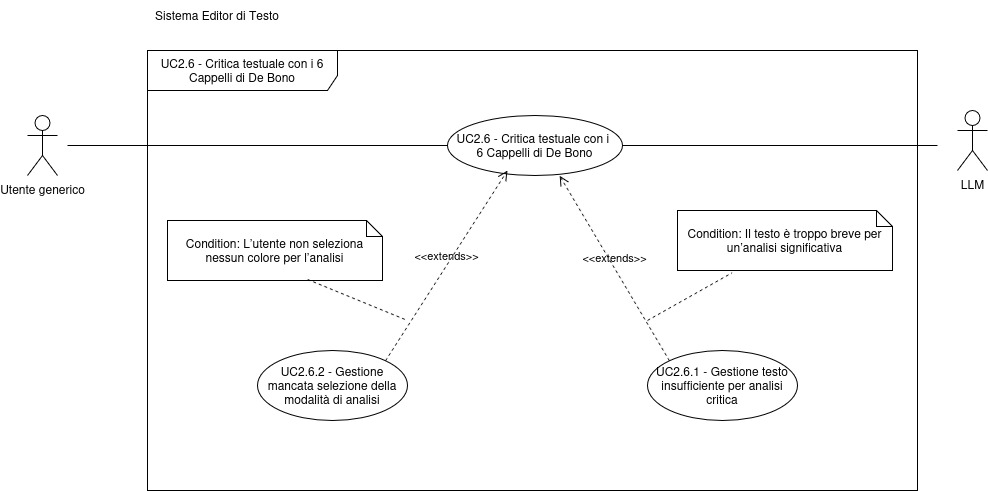
\includegraphics[width=0.8\textwidth]{../UCimg/UC2.6.jpg}
    \caption{Diagramma dei casi d'uso UC-2.6, 2.6.1, 2.6.2}
    \label{fig:uc2.6}
\end{figure}

\subsubsection{UC-2.6.3 - Critica testuale con il Cappello Bianco}
\begin{itemize}
    \item \textbf{Attore principale}: Utente generico
    \item \textbf{Descrizione}: Analisi oggettiva e fattuale del testo basata sul modello del Cappello Bianco di De Bono
    \item \textbf{Precondizioni}: È presente testo nell’editor
    \item \textbf{Postcondizioni}: Viene generata un’analisi fattuale inserita nel documento con formattazione distintiva
    \item \textbf{Scenario principale}:
    \begin{itemize}
        \item L’utente seleziona il testo da analizzare (o nessuna selezione per l'intero documento)
        \item L’utente clicca sul menu ”Analisi critica”
        \item L’utente imposta ”Cappello Bianco” come modalità di analisi
        \item Il sistema elabora la richiesta e invia il testo al LLM
        \item Il sistema genera l'analisi e la inserisce nell'editor, dopo il testo originale selezionato, applicando lo stile distintivo per il testo generato
    \end{itemize}
\end{itemize}

\subsubsection{UC-2.6.4 - Critica testuale con il Cappello Rosso}
\begin{itemize}
    \item \textbf{Attore principale}: Utente generico
    \item \textbf{Descrizione}: Analisi emotiva e intuitiva del testo basata sul modello del Cappello Rosso di De Bono
    \item \textbf{Precondizioni}: È presente testo nell’editor
    \item \textbf{Postcondizioni}: Viene generata un’analisi emotiva inserita nel documento con formattazione distintiva
    \item \textbf{Scenario principale}:
    \begin{itemize}
        \item L’utente seleziona il testo da analizzare (o nessuna selezione per l'intero documento)
        \item L’utente clicca sul menu ”Analisi critica”
        \item L’utente imposta ”Cappello Rosso” come modalità di analisi
        \item Il sistema elabora la richiesta e invia il testo al LLM
        \item Il sistema genera l'analisi e la inserisce nell'editor, dopo il testo originale selezionato, applicando lo stile distintivo per il testo generato
    \end{itemize}
\end{itemize}

\subsubsection{UC-2.6.5 - Critica testuale con il Cappello Nero}
\begin{itemize}
    \item \textbf{Attore principale}: Utente generico
    \item \textbf{Descrizione}: Analisi critica e cautelativa del testo basata sul modello del Cappello Nero di De Bono
    \item \textbf{Precondizioni}: È presente testo nell’editor
    \item \textbf{Postcondizioni}: Viene generata un’analisi critica inserita nel documento con formattazione distintiva
    \item \textbf{Scenario principale}:
    \begin{itemize}
        \item L’utente seleziona il testo da analizzare (o nessuna selezione per l'intero documento)
        \item L’utente clicca sul menu ”Analisi critica”
        \item L’utente imposta ”Cappello Nero” come modalità di analisi
        \item Il sistema elabora la richiesta e invia il testo al LLM
        \item Il sistema genera l'analisi e la inserisce nell'editor, dopo il testo originale selezionato, applicando lo stile distintivo per il testo generato
    \end{itemize}
\end{itemize}

\subsubsection{UC-2.6.6 - Critica testuale con il Cappello Giallo}
\begin{itemize}
    \item \textbf{Attore principale}: Utente generico
    \item \textbf{Descrizione}: Analisi ottimistica e costruttiva del testo basata sul modello del Cappello Giallo di De Bono
    \item \textbf{Precondizioni}: È presente testo nell’editor
    \item \textbf{Postcondizioni}: Viene generata un’analisi ottimistica inserita nel documento con formattazione distintiva
    \item \textbf{Scenario principale}:
    \begin{itemize}
        \item L’utente seleziona il testo da analizzare (o nessuna selezione per l'intero documento)
        \item L’utente clicca sul menu ”Analisi critica”
        \item L’utente imposta ”Cappello Giallo” come modalità di analisi
        \item Il sistema elabora la richiesta e invia il testo al LLM
        \item Il sistema genera l'analisi e la inserisce nell'editor, dopo il testo originale selezionato, applicando lo stile distintivo per il testo generato
    \end{itemize}
\end{itemize}

\subsubsection{UC-2.6.7 - Critica testuale con il Cappello Verde}
\begin{itemize}
    \item \textbf{Attore principale}: Utente generico
    \item \textbf{Descrizione}: Analisi creativa e innovativa del testo basata sul modello del Cappello Verde di De Bono
    \item \textbf{Precondizioni}: È presente testo nell’editor
    \item \textbf{Postcondizioni}: Viene generata un’analisi creativa inserita nel documento con formattazione distintiva
    \item \textbf{Scenario principale}:
    \begin{itemize}
        \item L’utente seleziona il testo da analizzare (o nessuna selezione per l'intero documento)
        \item L’utente clicca sul menu ”Analisi critica”
        \item L’utente imposta ”Cappello Verde” come modalità di analisi
        \item Il sistema elabora la richiesta e invia il testo al LLM
        \item Il sistema genera l'analisi e la inserisce nell'editor, dopo il testo originale selezionato, applicando lo stile distintivo per il testo generato
    \end{itemize}
\end{itemize}

\subsubsection{UC-2.6.8 - Critica testuale con il Cappello Blu}
\begin{itemize}
    \item \textbf{Attore principale}: Utente generico
    \item \textbf{Descrizione}: Analisi processuale e organizzativa del testo basata sul modello del Cappello Blu di De Bono
    \item \textbf{Precondizioni}: È presente testo nell’editor
    \item \textbf{Postcondizioni}: Viene generata un’analisi processuale inserita nel documento con formattazione distintiva
    \item \textbf{Scenario principale}:
    \begin{itemize}
        \item L’utente seleziona il testo da analizzare (o nessuna selezione per l'intero documento)
        \item L’utente clicca sul menu ”Analisi critica”
        \item L’utente imposta ”Cappello Blu” come modalità di analisi
        \item Il sistema elabora la richiesta e invia il testo al LLM
        \item Il sistema genera l'analisi e la inserisce nell'editor, dopo il testo originale selezionato, applicando lo stile distintivo per il testo generato
    \end{itemize}
\end{itemize}

\begin{figure}[H]
    \centering
    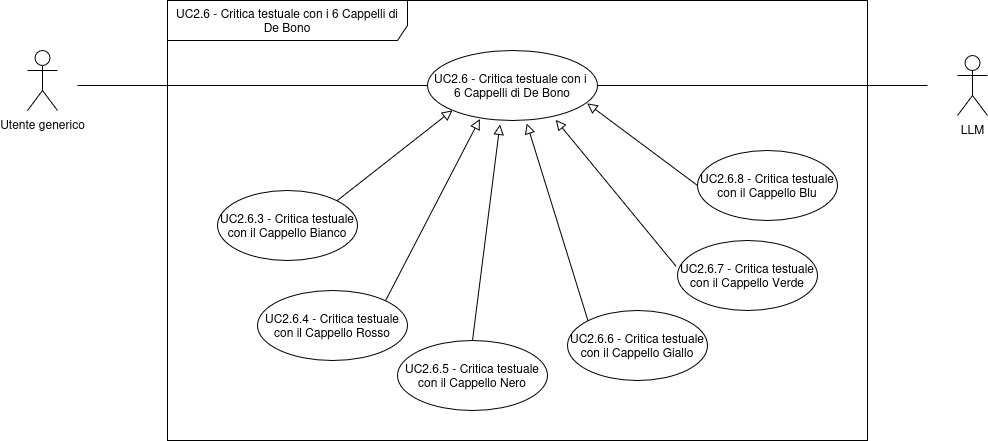
\includegraphics[width=0.8\textwidth]{../UCimg/UC2.6.3.jpg}
    \caption{Diagramma dei casi d'uso UC-2.6.3 - 2.6.8}
    \label{fig:uc2.6.3}
\end{figure}

\subsubsection{UC-2.7 - Generazione di testo (Distant Writing)}
\begin{itemize}
    \item \textbf{Attore principale}: Utente generico
    \item \textbf{Descrizione}: Creazione di nuovo testo inedito a partire da un prompt descrittivo fornito dall’utente
    \item \textbf{Precondizioni}: L’editor è aperto e pronto per la scrittura
    \item \textbf{Postcondizioni}: Viene generato un nuovo testo basato sul prompt e inserito nell’editor con la formattazione distintiva del testo AI
    \item \textbf{Scenario principale}:
    \begin{itemize}
        \item L’utente si posiziona nel punto del documento dove vuole inserire il testo generato
        \item L’utente inserisce un prompt descrivendo il contenuto desiderato (tramite chatbox o comando rapido)
        \item Il sistema invia il prompt al LLM
        \item Il sistema inserisce nell'editor il testo generato nel punto indicato, applicando lo stile distintivo per il testo generato
    \end{itemize}
    \item \textbf{Estensioni}:
    \begin{itemize}
        \item L’utente fornisce un prompt troppo vago o incompleto
    \end{itemize}
\end{itemize}

\subsubsection{UC-2.7.1 - Gestione prompt incompleto}
\begin{itemize}
    \item \textbf{Attore principale}: Utente generico
    \item \textbf{Descrizione}: Il sistema rileva una richiesta poco chiara o incompleta e guida l'utente nel miglioramento del prompt prima di invocare l'AI
    \item \textbf{Precondizioni}: L'utente ha avviato una richiesta di generazione testo (Distant Writing)
    \item \textbf{Postcondizioni}: La generazione viene sospesa e all'utente vengono forniti suggerimenti operativi per affinare la richiesta
    \item \textbf{Scenario principale}:
    \begin{itemize}
        \item L’utente si posiziona nel punto del documento dove vuole inserire il testo generato
        \item L’utente inserisce un prompt descrivendo il contenuto desiderato (tramite chatbox o comando rapido)
        \item LLM analizza il prompt e lo valuta come troppo vago, breve o privo di contesto sufficiente
        \item Il sistema interrompe la richiesta e mostra un messaggio di avviso chiedendo chiarimenti
        \item Il sistema propone esempi di prompt efficaci o template basati sul contesto corrente (opzionale)
        \item Il sistema rimane in attesa di un nuovo input migliorativo da parte dell'utente
    \end{itemize}
\end{itemize}

\begin{figure}[H]
    \centering
    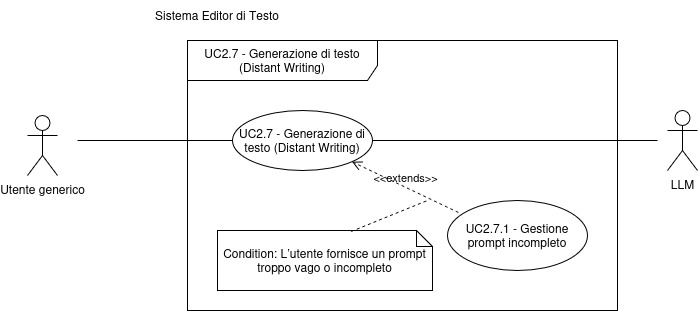
\includegraphics[width=0.8\textwidth]{../UCimg/UC2.7.jpg}
    \caption{Diagramma dei casi d'uso UC-2.7, 2.7.1}
    \label{fig:uc2.7}
\end{figure}

\subsubsection{UC-2.8 - Generazione di grafici e tabelle}
\begin{itemize}
    \item \textbf{Attore principale}: Utente generico
    \item \textbf{Descrizione}: Creazione automatica di rappresentazioni visive (grafici o tabelle) basate su dati descritti nel testo
    \item \textbf{Precondizioni}: È presente testo descrittivo contenente dati nell’editor
    \item \textbf{Postcondizioni}: Viene generato un elemento grafico o tabellare inserito nel documento con formattazione distintiva
    \item \textbf{Scenario principale}:
    \begin{itemize}
    \item L’utente seleziona la porzione di testo contenente i dati
    \item L’utente attiva il comando ”Genera grafico/tabella”
    \item L’utente specifica il tipo di visualizzazione desiderata (es. tabella, grafico a barre, torta)
    \item Il sistema elabora la richiesta e invia i dati al LLM
    \item Il sistema genera l'elemento visivo e lo inserisce nell'editor, dopo il testo selezionato, applicando lo stile distintivo per il contenuto generato
    \end{itemize}
    \item \textbf{Estensioni}:
    \begin{itemize}
        \item Il testo non contiene dati strutturati sufficienti
    \end{itemize}
\end{itemize}

\subsubsection{UC-2.8.1 - Gestire dati insufficienti per la visualizzazione di grafici e tabelle}
\begin{itemize}
    \item \textbf{Attore principale}: Utente generico
    \item \textbf{Descrizione}: Il sistema rileva l'impossibilità di creare un grafico o una tabella a causa della mancanza di dati strutturati nel testo selezionato
    \item \textbf{Precondizioni}: L’utente ha attivato il comando di generazione grafico/tabella su una selezione di testo
    \item \textbf{Postcondizioni}: L’operazione viene annullata e viene mostrato un messaggio di avviso. Il testo originale rimane invariato
    \item \textbf{Scenario principale}:
    \begin{itemize}
        \item L'utente attiva il comando "Genera grafico/tabella" su una porzione di testo
        \item Il sistema elabora la richiesta e invia i dati al LLM
        \item LLM analizza il contenuto selezionato per estrarre serie di dati
        \item LLM rileva che il testo è puramente descrittivo o privo di valori numerici/categorici sufficienti per una rappresentazione visiva
        \item Il sistema interrompe la generazione dell'elemento visivo
        \item Il sistema mostra un avviso all'utente
        \item Il testo originale rimane invariato
    \end{itemize}
\end{itemize}

\begin{figure}[H]
    \centering
    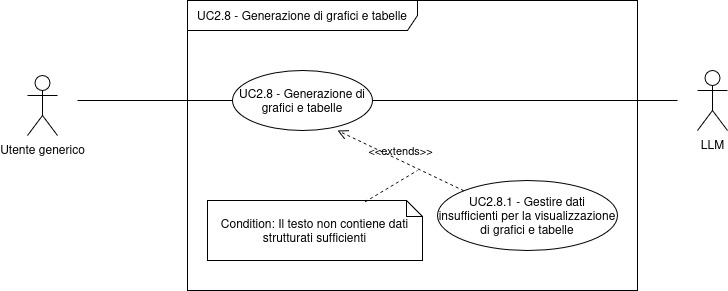
\includegraphics[width=0.8\textwidth]{../UCimg/UC2.8.jpg}
    \caption{Diagramma dei casi d'uso UC-2.8, 2.8.1}
    \label{fig:uc2.8}
\end{figure}

\subsubsection{UC-2.9 - Generazione di mappe concettuali}
\begin{itemize}
    \item \textbf{Attore principale}: Utente generico
    \item \textbf{Descrizione}: Creazione automatica di mappe concettuali per visualizzare le relazioni logiche tra i concetti presenti nel testo
    \item \textbf{Precondizioni}: È presente testo nell’editor (completo o selezionato)
    \item \textbf{Postcondizioni}: Viene generata una mappa concettuale che viene inserita nel documento
    \item \textbf{Scenario principale}:
    \begin{itemize}
        \item L’utente seleziona il testo da visualizzare come mappa (o nessuna selezione per l'intero documento)
        \item L’utente attiva il comando ”Genera mappa concettuale”
        \item Il sistema elabora la richiesta e invia il testo al LLM
        \item Il sistema renderizza la mappa concettuale e la inserisce nell'editor, applicando lo stile distintivo per il contenuto generato
    \end{itemize}
    \item \textbf{Estensioni}:
    \begin{itemize}
        \item Errore di visualizzazione o generazione della mappa
    \end{itemize}
\end{itemize}

\subsubsection{UC-2.9.1 - Gestione errori di visualizzazione delle mappe concettuali generate}
\begin{itemize}
    \item \textbf{Attore principale}: Utente generico
    \item \textbf{Descrizione}: Il sistema gestisce il fallimento del rendering grafico della mappa concettuale fornendo il codice sorgente utilizzabile esternamente
    \item \textbf{Precondizioni}: L’utente ha attivato la generazione di una mappa concettuale
    \item \textbf{Postcondizioni}: Il codice sorgente della mappa viene inserito nel documento al posto della rappresentazione grafica
    \item \textbf{Scenario principale}:
    \begin{itemize}
        \item Il sistema tenta di renderizzare la mappa concettuale generata dal LLM
        \item Il sistema rileva un errore di visualizzazione o una incompatibilità tecnica
        \item Il sistema mostra un avviso all'utente
        \item Il sistema inserisce nel documento il blocco di codice sorgente eseguibile (es. sintassi Mermaid o Graphviz) generato dal LLM, permettendo all'utente di generarla con strumenti esterni
    \end{itemize}
\end{itemize}

\begin{figure}[H]
    \centering
    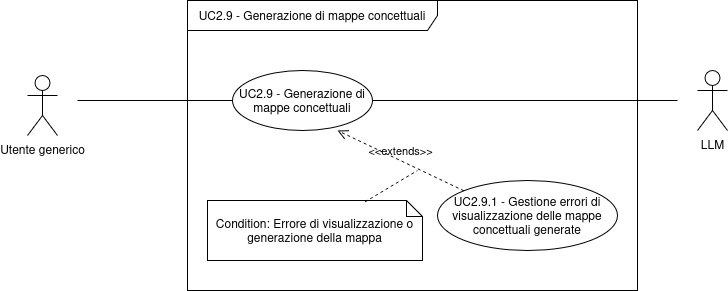
\includegraphics[width=0.8\textwidth]{../UCimg/UC2.9.jpg}
    \caption{Diagramma dei casi d'uso UC-2.9, 2.9.1}
    \label{fig:uc2.9}
\end{figure}

\subsubsection{UC-2.10 - Generazione di formule matematiche}
\begin{itemize}
    \item \textbf{Attore principale}: Utente generico
    \item \textbf{Descrizione}: Conversione automatica di descrizioni testuali di problemi matematici in formule formattate
    \item \textbf{Precondizioni}: È presente testo descrittivo di un problema matematico nell’editor
    \item \textbf{Postcondizioni}: Vengono generate le formule matematiche corrispondenti e inserite nel documento con formattazione distintiva
    \item \textbf{Scenario principale}:
    \begin{itemize}
    \item L’utente seleziona il testo descrittivo del problema
    \item L’utente attiva il comando ”Genera formule”
    \item Il sistema elabora la richiesta e invia il testo al LLM
    \item Il sistema genera il codice matematico (simile LaTeX) e lo inserisce nell'editor renderizzandolo, applicando lo stile distintivo per il contenuto generato
    \end{itemize}
    \item \textbf{Estensioni}:
    \begin{itemize}
        \item Il sistema non supporta simboli matematici complessi
    \end{itemize}
\end{itemize}

\subsubsection{UC-2.10.1 - Gestire simboli non supportati}
\begin{itemize}
    \item \textbf{Attore principale}: Utente generico
    \item \textbf{Descrizione}: Il sistema gestisce la presenza di notazioni matematiche complesse non supportate dal motore di rendering locale
    \item \textbf{Precondizioni}: L’utente ha attivato la generazione di formule matematiche
    \item \textbf{Postcondizioni}: La formula viene inserita come codice grezzo o testo approssimato invece che renderizzata graficamente
    \item \textbf{Scenario principale}:
    \begin{itemize}
        \item Il sistema analizza l'output matematico generato dal LLM
        \item Il sistema identifica simboli o costrutti non supportati dal motore di rendering integrato
        \item Il sistema segnala la limitazione all'utente tramite un avviso
        \item Il sistema inserisce la formula in formato codice grezzo o in una rappresentazione testuale approssimata, applicando lo stile distintivo per il contenuto generato
    \end{itemize}
\end{itemize}

\begin{figure}[H]
    \centering
    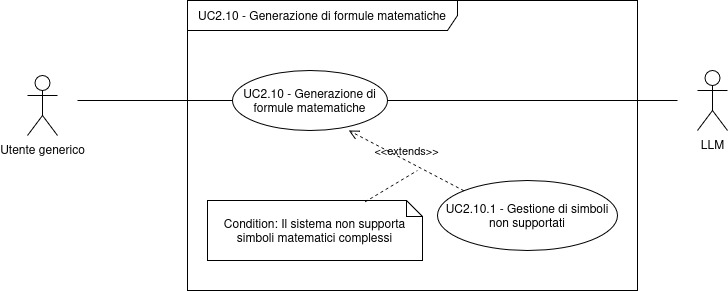
\includegraphics[width=0.8\textwidth]{../UCimg/UC2.10.jpg}
    \caption{Diagramma dei casi d'uso UC-2.10, 2.10.1}
    \label{fig:uc2.10}
\end{figure}

\newpage

\subsection{Macroarea 3 - Persistenza: Caricamento}
\subsubsection{UC-3.0 - Caricamento file}
\begin{itemize}
    \item \textbf{Attore principale}: Utente generico
    \item \textbf{Descrizione}: Permettere all'utente di caricare un documento nell'editor
    \item \textbf{Precondizioni}: L'utente ha un file che vuole caricare nell'editor
    \item \textbf{Postcondizioni}: L'utente ha caricato con successo il file nell'editor
    \item \textbf{Scenario principale}:
        \begin{itemize}
            \item Utente vuole caricare un file
            \item Utente clicca il pulsante per caricare il file
            \item Utente sceglie tra due opzioni: trascina file e esplora file
            \item Utente carica il documento
        \end{itemize}
    \item \textbf{Estensioni}:
        \begin{itemize}
            \item Utente seleziona un file non supportato
            \item Utente seleziona un file troppo grande
        \end{itemize}
\end{itemize}

\subsubsection{UC-3.0.1 - Opzione trascina file}
\begin{itemize}
    \item \textbf{Attore principale}: Utente generico
    \item \textbf{Descrizione}: Utente trascina il file nella finestra per caricare file
    \item \textbf{Precondizioni}: Utente clicca tasto per trascinare file
    \item \textbf{Postcondizioni}: Utente ha trascinato file
    \item \textbf{Scenario principale}:
        \begin{itemize}
            \item Utente sceglie opzione trascina file
            \item Utente trascina file
            \item Utente ha caricato il file
        \end{itemize}
\end{itemize}

\subsubsection{UC-3.0.2 - Opzione esplora file}
\begin{itemize}
    \item \textbf{Attore principale}: Utente generico
    \item \textbf{Descrizione}: Utente vede i propri file e ne sceglie uno da caricare
    \item \textbf{Precondizioni}: Utente clicca tasto per aprire esplora file
    \item \textbf{Postcondizioni}: Utente ha scelto un file
    \item \textbf{Scenario principale}:
        \begin{itemize}
            \item Utente sceglie opzione esplora file
            \item Utente trascina file
            \item Utente ha caricato il file
        \end{itemize}
\end{itemize}

\begin{figure}[H]
    \centering
    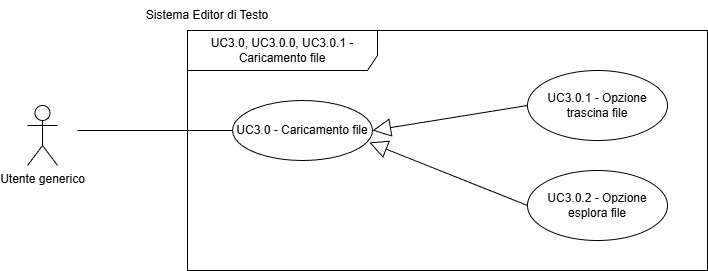
\includegraphics[width=0.8\textwidth]{../UCimg/UC3.0.jpg}
    \caption{Diagramma dei casi d'uso UC-3.0, 3.0.1, 3.0.2}
    \label{fig:uc3.0}
\end{figure}

\subsubsection{UC-3.1 - Gestione formati file non supportati}
\begin{itemize}
    \item \textbf{Attore principale}: Utente generico
    \item \textbf{Descrizione}: L'utente prova a caricare un documento ma è di un formato non supportato
    \item \textbf{Precondizioni}: Il file caricato è di un formato non supportato
    \item \textbf{Postcondizioni}: Appare il messaggio di errore "Formato non supportato"
    \item \textbf{Scenario principale}:
        \begin{itemize}
            \item L'utente seleziona un file tramite "Esplora file" o lo trascina nell'area di caricamento
            \item Il sistema analizza il tipo del file selezionato
            \item Il sistema rileva che il formato non è tra quelli supportati
            \item Il sistema blocca il processo di caricamento
            \item Viene visualizzato a schermo un messaggio di errore
        \end{itemize}
\end{itemize}

\subsubsection{UC-3.2 - Gestione file troppo grandi}
\begin{itemize}
    \item \textbf{Attore principale}: Utente generico
    \item \textbf{Descrizione}: L'utente prova a caricare un documento ma è di dimensioni troppo grandi
    \item \textbf{Precondizioni}: Il file caricato è di dimensioni troppo grandi
    \item \textbf{Postcondizioni}: Appare il messaggio di errore "File troppo grande"
    \item \textbf{Scenario principale}:
        \begin{itemize}
            \item L'utente seleziona un file tramite "Esplora file" o lo trascina nell'area di caricamento
            \item Il sistema controlla la dimensione del file
            \item Il sistema rileva che la dimensione del file supera il limite massimo consentito
            \item Il sistema blocca il processo di caricamento
            \item Viene visualizzato a schermo un messaggio di errore
        \end{itemize}
\end{itemize}

\subsubsection{UC-3.3 - Rimozione file caricato}
\begin{itemize}
    \item \textbf{Attore principale}: Utente generico
    \item \textbf{Descrizione}: utente vuole rimuovere un file che ha caricato
    \item \textbf{Precondizioni}: utente clicca tasto per rimuovere file caricato
    \item \textbf{Postcondizioni}: utente ha rimosso con successo il file
    \item \textbf{Scenario principale}:
        \begin{itemize}
            \item Utente clicca il pulsante rimuovi file
            \item Utente vede la schermata “Sei sicuro di voler rimuovere?”
            \item Utente preme si e rimuove con successo il file
        \end{itemize}
        \item \textbf{Estensioni}:
        \begin{itemize}
            \item Utente clicca no nella schermata “Sei sicuro di voler rimuovere?” e quindi il file non viene rimosso
        \end{itemize}
\end{itemize}

\subsubsection{UC-3.3.1 - Annullamento rimozione file caricato}
\begin{itemize}
    \item \textbf{Attore principale}: Utente generico
    \item \textbf{Descrizione}: utente annulla la rimozione di un file che ha caricato
    \item \textbf{Precondizioni}: utente clicca tasto tasto no nella schermata "Sei sicuro di voler rimuovere?"
    \item \textbf{Postcondizioni}: il file non viene rimosso
    \item \textbf{Scenario principale}:
        \begin{itemize}
            \item Utente clicca l'opzione no nella schermata "Sei sicuro di voler rimuovere?"
            \item La rimozione del file viene annullata
            \item L'utente torna nella pagina del file che ha caricato
        \end{itemize}
\end{itemize}

\begin{figure}[H]
    \centering
    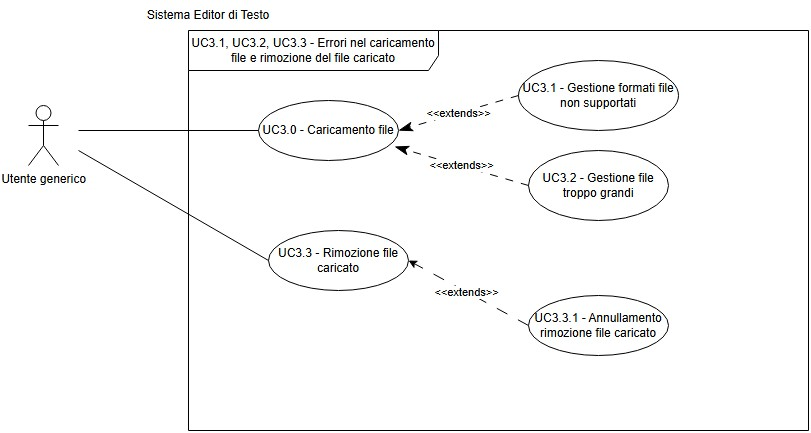
\includegraphics[width=0.8\textwidth]{../UCimg/UC3.1_3.2_3.jpg}
    \caption{Diagramma dei casi d'uso UC-3.1, 3.2, 3.3}
    \label{fig:uc3.1}
\end{figure}

\newpage

\subsection{Macroarea 4 - Persistenza: Salvataggio}
\subsubsection{UC-4.0 - Esportazione di un file}
\begin{itemize}
    \item \textbf{Attore principale}: Utente generico
    \item \textbf{Descrizione}: Permettere all'utente di esportare il documento su cui ha lavorato
    \item \textbf{Precondizioni}: Testo scritto nell'editor di testo
    \item \textbf{Postcondizioni}: L'utente ha il documento salvato in locale
    \item \textbf{Scenario principale}:
        \begin{itemize}
            \item Utente scrive del testo
            \item Utente decide di esportare il documento
            \item Utente preme sul tasto esporta
            \item Utente può selezionare il formato con cui esportare il file e le pagine che vuole esportare
        \end{itemize}
\end{itemize}

\subsubsection{UC-4.0.1 - Esportare un file in PDF}
\begin{itemize}
    \item \textbf{Attore principale}: Utente generico
    \item \textbf{Descrizione}: Testo compilato salvato in locale sulla propria macchina in formato PDF
    \item \textbf{Precondizioni}: L'utente ha un documento che desidera scaricare
    \item \textbf{Postcondizioni}: L'utente ottiene un documento in formato PDF salvato localmente
    \item \textbf{Scenario principale}:
        \begin{itemize}
            \item Utente seleziona l'opzione "PDF" tra le opzioni di esportazione
            \item Il documento viene convertito in formato PDF
            \item Utente ottiene il documento salvato in PDF
        \end{itemize}
\end{itemize}

\subsubsection{UC-4.0.2 - Esportare un file in MD}
\begin{itemize}
    \item \textbf{Attore principale}: Utente generico
    \item \textbf{Descrizione}: Testo compilato salvato in locale sulla propria macchina in formato testuale
    \item \textbf{Precondizioni}: L'utente ha un documento che desidera scaricare
    \item \textbf{Postcondizioni}: L'utente ottiene un documento in formato MD salvato localmente
    \item \textbf{Scenario principale}:
        \begin{itemize}
            \item Utente seleziona opzione "src" tra le opzioni di esportazione
            \item Il documento viene salvato in formato MD
        \end{itemize}
\end{itemize}

\subsubsection{UC-4.0.3 - Esportare un file in formato HTML}
\begin{itemize}
    \item \textbf{Attore principale}: Utente generico
    \item \textbf{Descrizione}: Genera del codice HTML dal testo Markdown
    \item \textbf{Precondizioni}: L'utente ha un documento non vuoto
    \item \textbf{Postcondizioni}: L'utente ottiene un file .HTML in cui viene convertito il testo Markdown in codice HTML
    \item \textbf{Scenario principale}:
        \begin{itemize}
            \item Utente seleziona opzione "HTML" tra le opzioni di esportazione
            \item Il documento viene convertito in formato HTML
            \item Utente riceve il documento in formato HTML
        \end{itemize}
\end{itemize}

\subsubsection{UC-4.0.4 - Esportare un file in formato ODT}
\begin{itemize}
    \item \textbf{Attore principale}: Utente generico
    \item \textbf{Descrizione}: Genera documenti compatibili con popolari editor testuali
    \item \textbf{Precondizioni}: L'utente ha un documento non vuoto
    \item \textbf{Postcondizioni}: L'utente ottiene un file .ODT salvato localmente
    \item \textbf{Scenario principale}:
        \begin{itemize}
            \item Utente seleziona opzione "ODT" tra le opzioni di esportazione
            \item Il documento viene convertito in formato ODT
            \item Utente riceve il documento in formato ODT
        \end{itemize}
\end{itemize}

\subsubsection{UC-4.0.5 - Esportare un file in formato DOCX}
\begin{itemize}
    \item \textbf{Attore principale}: Utente generico
    \item \textbf{Descrizione}: Genera documenti compatibili con Microsoft Word
    \item \textbf{Precondizioni}: L'utente ha un documento non vuoto
    \item \textbf{Postcondizioni}: L'utente ottiene un file .DOCX salvato localmente
    \item \textbf{Scenario principale}:
        \begin{itemize}
            \item Utente seleziona opzione "DOCX" tra le opzioni di esportazione
            \item Il documento viene convertito in formato DOCX
            \item Utente riceve il documento in formato DOCX
        \end{itemize}
\end{itemize}
\begin{figure}[H]
    \centering
    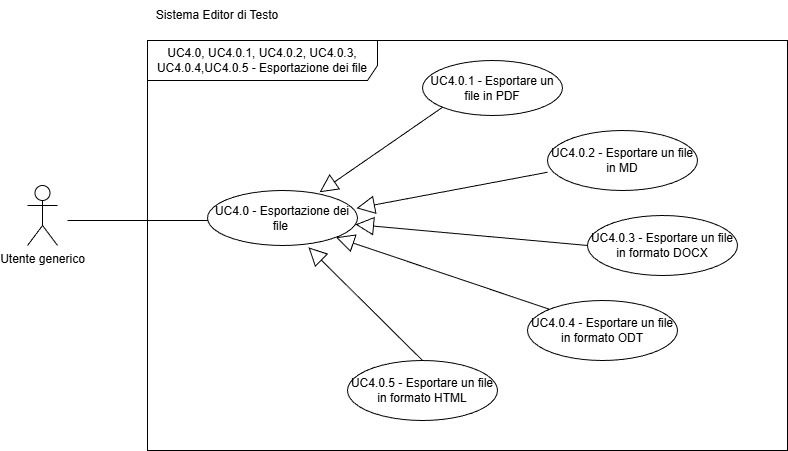
\includegraphics[width=0.8\textwidth]{../UCimg/UC4.0.jpg}
    \caption{Diagramma dei casi d'uso UC-4.0, UC-4.0.1, UC-4.0.2, UC-4.0.3, UC-4.0.4, UC-4.0.5*}
    \label{fig:uc4.0}
\end{figure}

\subsubsection{UC-4.1 - Esportare selezionate pagine del documento}
\begin{itemize}
    \item \textbf{Attore principale}: Utente generico
    \item \textbf{Descrizione}: Scaricare nel formato desiderato solo alcune pagine del documento
    \item \textbf{Precondizioni}: L'utente ha un documento non vuoto, con diverse pagine
    \item \textbf{Postcondizioni}: L'utente ottiene un file in formato a scelta con solo le pagine selezionate
    \item \textbf{Scenario principale}:
        \begin{itemize}
            \item Utente vuole scaricare solo selezionate pagine del documento da salvare
            \item Tra le opzioni di esportazione, elenca numericamente le pagine desiderate
            \item Seleziona modalità di esportazione
            \item Ottiene le pagine selezionate in un nuovo documento, salvato nel formato selezionato
        \end{itemize}
    \item \textbf{Estensioni}:
        \begin{itemize}
            \item L'utente esporta un range di pagine del documento
        \end{itemize}
\end{itemize}

\subsubsection{UC-4.1.1 - Esportare un range di pagine del documento}
\begin{itemize}
    \item \textbf{Attore principale}: Utente generico
    \item \textbf{Descrizione}: Scaricare nel formato desiderato solo un range di pagine del documento
    \item \textbf{Precondizioni}: L'utente ha un documento non vuoto, con diverse pagine
    \item \textbf{Postcondizioni}: L'utente ottiene un file in formato a scelta con solo il range di pagine selezionate
    \item \textbf{Scenario principale}:
        \begin{itemize}
            \item Utente vuole scaricare porzioni consecutive di un documento
            \item Utente seleziona la pagina di inizio e fine del range da scaricare
            \item Seleziona modalità di esportazione
            \item Ottiene le pagine selezionate in un nuovo documento, salvato nel formato selezionato
        \end{itemize}
\end{itemize}
\begin{figure}[H]
    \centering
    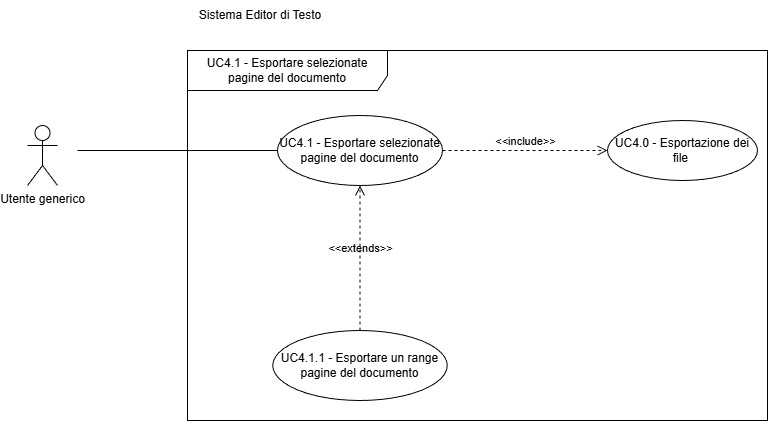
\includegraphics[width=0.8\textwidth]{../UCimg/UC4.1.jpg}
    \caption{Diagramma dei casi d'uso UC-4.1, UC-4.1.1}
    \label{fig:uc4.2}
\end{figure}

\subsubsection{UC-4.2 - Stampare il documento}
\begin{itemize}
    \item \textbf{Attore principale}: Utente generico
    \item \textbf{Descrizione}: Utente desidera stampare il documento senza doverlo prima esportare
    \item \textbf{Precondizioni}: L'utente ha un documento aperto
    \item \textbf{Postcondizioni}: L'utente ottiene il documento stampato
    \item \textbf{Scenario principale}:
        \begin{itemize}
            \item Utente ha un documento aperto che desidera stampare
            \item Utente preme un pulsante "stampa"
            \item Utente ha accesso alle opzioni di stampa offerte dal suo browser
            \item Utente ritorna al proprio documento una volta completata l'operazione
        \end{itemize}
    \item \textbf{Estensioni}:
        \begin{itemize}
            \item L'utente stampa solo selezionate pagine del documento
        \end{itemize}
\end{itemize}

\subsubsection{UC-4.2.1 - Stampare selezionate pagine del documento}
\begin{itemize}
    \item \textbf{Attore principale}: Utente generico
    \item \textbf{Descrizione}: Utente desidera stampare solo alcune pagine del documento
    \item \textbf{Precondizioni}: L'utente ha un documento aperto
    \item \textbf{Postcondizioni}: L'utente ottiene il documento stampato
    \item \textbf{Scenario principale}:
        \begin{itemize}
            \item Utente ha un documento aperto che desidera stampare
            \item Utente preme un pulsante "stampa"
            \item Utente ha accesso alle opzioni di stampa offerte dal suo browser
            \item Utente ha la possibilità di selezionare le pagine che desidera stampare
            \item Utente ritorna al proprio documento una volta completata l'operazione
        \end{itemize}
\end{itemize}
\begin{figure}[H]
    \centering
    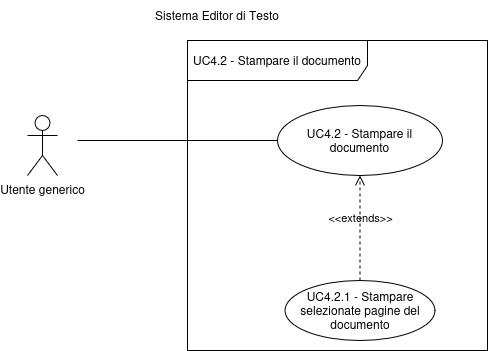
\includegraphics[width=0.8\textwidth]{../UCimg/UC4.2.jpg}
    \caption{Diagramma dei casi d'uso UC-4.2, UC-4.2.1}
    \label{fig:uc4.3}
\end{figure}

\newpage

\subsection{Macroarea 5 - Autenticazione}
\subsubsection{UC-5.0 - Login}
\begin{itemize}
    \item \textbf{Attore principale}: Utente non autenticato
    \item \textbf{Descrizione}: Permette all'utente di accedere al proprio account, rendendo così disponibili funzionalità di salvataggio, modifica e cancellazione di documenti nel db, salvati a nome dell'utente
    \item \textbf{Precondizioni}: L'utente è già registrato presso il sistema
    \item \textbf{Postcondizioni}: All'utente è permesso accedere al suo account nel sistema
    \item \textbf{Scenario principale}:
        \begin{itemize}
            \item L'utente accede al sistema
            \item L'utente seleziona la funzionalità Login
            \item L'utente inserisce un username ed una password univoci nel sistema
            \item All'utente viene permesso l'accesso
        \end{itemize}
    \item \textbf{Estensioni}:
        \begin{itemize}
            \item L'utente inserisce un username non presente nel db
            \item L'utente inserisce un username esistente ma la password sbagliata
        \end{itemize}
\end{itemize}

\subsubsection{UC-5.0.1 - Gestione username inesistente}
\begin{itemize}
    \item \textbf{Attore principale}: Utente non autenticato
    \item \textbf{Descrizione}: Il sistema gestisce il tentativo di accesso con un identificativo utente non presente nel database
    \item \textbf{Precondizioni}: L’utente ha inviato una richiesta di login
    \item \textbf{Postcondizioni}: L’accesso viene negato e viene mostrato un messaggio di errore specifico
    \item \textbf{Scenario principale}:
    \begin{itemize}
        \item Il sistema interroga il database alla ricerca dell'username fornito
        \item Il sistema non rileva alcuna corrispondenza (account inesistente)
        \item Il sistema nega l'accesso
        \item Il sistema mostra all’utente un messaggio di avviso
        \item L'utente rimane nella schermata di login
    \end{itemize}
\end{itemize}

\subsubsection{UC-5.0.2 - Gestione password errata}
\begin{itemize}
    \item \textbf{Attore principale}: Utente non autenticato
    \item \textbf{Descrizione}: Il sistema gestisce il tentativo di accesso con un username valido ma associato a una password non corrispondente
    \item \textbf{Precondizioni}: L’utente ha inviato una richiesta di login con un username esistente
    \item \textbf{Postcondizioni}: L’accesso viene negato e viene mostrato un messaggio di errore specifico
    \item \textbf{Scenario principale}:
    \begin{itemize}
        \item Il sistema rileva che l'username esiste
        \item Il sistema verifica la corrispondenza crittografica della password inserita con quella memorizzata
        \item Il sistema rileva una incongruenza
        \item Il sistema nega l'accesso
        \item Il sistema mostra all’utente un messaggio di avviso
        \item L'utente rimane nella schermata di login
    \end{itemize}
\end{itemize}

\subsubsection{UC-5.1 - Registrazione}
\begin{itemize}
    \item \textbf{Attore principale}: Utente non autenticato
    \item \textbf{Descrizione}: L'utente potrà creare un nuovo account nel sistema accedendo così alle funzionalità di salvataggio, modifica e cancellazione di documenti nel db, salvati a nome dell'utente
    \item \textbf{Precondizioni}: L'utente non è ancora autenticato nel sistema
    \item \textbf{Postcondizioni}: L'utente possiede un account nel sistema individuato da un username ed una password
    \item \textbf{Scenario principale}:
        \begin{itemize}
            \item L'utente accede al sistema
            \item L'utente seleziona la funzionalità "Registrati"
            \item L'utente inserisce un username univoco nel sistema
            \item L'utente inserisce una password che rispetta i vincoli
        \end{itemize}
    \item \textbf{Estensioni}:
        \begin{itemize}
            \item L'utente inserisce un username già esistente nel sistema
        \end{itemize}
\end{itemize}

\subsubsection{UC-5.1.1 - Gestione username già esistente}
\begin{itemize}
\item \textbf{Attore principale}: Utente non autenticato
\item \textbf{Descrizione}: Il sistema impedisce la creazione di un account duplicato se l'identificativo scelto è già presente nel database
\item \textbf{Precondizioni}: L’utente ha inviato i dati per la registrazione
\item \textbf{Postcondizioni}: La registrazione viene bloccata e l'utente viene avvisato
\item \textbf{Scenario principale}:
\begin{itemize}
\item Il sistema controlla la disponibilità dell'username (o email) nel database
\item Il sistema rileva che l'username è già associato a un account esistente
\item Il sistema blocca la creazione del nuovo record
\item Il sistema visualizza un messaggio di errore
\item L'utente viene riportato al modulo di login
\end{itemize}
\end{itemize}

\begin{figure}[H]
    \centering
    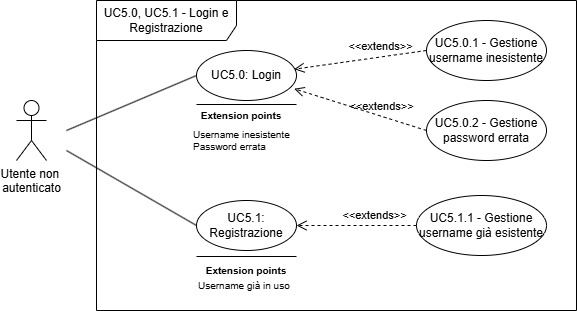
\includegraphics[width=0.8\textwidth]{../UCimg/UC5.0.jpg}
    \caption{Diagramma dei casi d'uso UC-5.0, 5.0.*, 5.1, 5.1.*}
    \label{fig:uc5.0}
\end{figure}


\subsubsection{UC-5.2 - Eliminazione dell'account}
\begin{itemize}
    \item \textbf{Attore principale}: Utente autenticato
    \item \textbf{Descrizione}: L'utente decide di eliminare il proprio account dal sistema
    \item \textbf{Precondizioni}: L'utente è autenticato nel sistema
    \item \textbf{Postcondizioni}: L'account dell'utente viene eliminato dal sistema e l'utente non potrà più accedere alle funzionalità relative alle sue note
    \item \textbf{Scenario principale}:
        \begin{itemize}
            \item L'utente accede al sistema
            \item L'utente seleziona l'opzione "Elimina account"
            \item Il sistema mostra un pop up di conferma della scelta
            \item L'utente accetta e viene sloggato
            \item Il sistema elimina dal db il nome utente e la password relative all'attore
        \end{itemize}
    \item \textbf{Estensioni}:
        \begin{itemize}
            \item L'utente seleziona "annulla" nel pop up di conferma
        \end{itemize}
\end{itemize}

\subsubsection{UC-5.2.1 - Annullamento della procedura di eliminazione account}
\begin{itemize}
    \item \textbf{Attore principale}: Utente autenticato
    \item \textbf{Descrizione}: Il sistema gestisce l'interruzione della procedura di eliminazione su richiesta dell'utente
    \item \textbf{Precondizioni}: È visualizzata la richiesta di conferma per l'eliminazione dell'account
    \item \textbf{Postcondizioni}: La procedura viene interrotta, l'account rimane attivo e i dati intatti
    \item \textbf{Scenario principale}:
    \begin{itemize}
        \item L’utente, di fronte alla richiesta di conferma, seleziona l’opzione ”Annulla” (o chiude il popup)
        \item Il sistema chiude la finestra di dialogo
        \item Il sistema abortisce l'operazione di cancellazione sul database
        \item L'utente viene riportato alla schermata delle impostazioni del profilo nello stato precedente
    \end{itemize}
\end{itemize}

\begin{figure}[H]
    \centering
    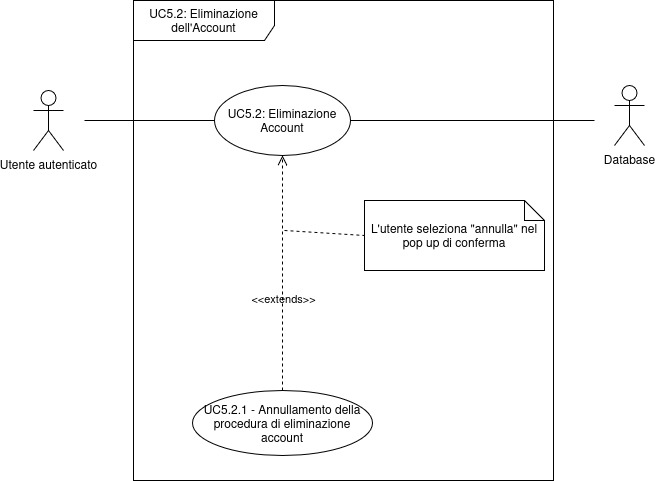
\includegraphics[width=0.8\textwidth]{../UCimg/UC5.2.jpg}
    \caption{Diagramma dei casi d'uso UC-5.2, 5.2.1}
    \label{fig:uc5.2}
\end{figure}


\subsubsection{UC-5.3 - Apertura file recenti}
\begin{itemize}
    \item \textbf{Attore principale}: Utente autenticato
    \item \textbf{Descrizione}: L'utente vuole aprire un file dal db creato in precedenza
    \item \textbf{Precondizioni}: L'utente è autenticato nel sistema
    \item \textbf{Postcondizioni}: L'utente continua a lavorare su una nota precedentemente salvata
    \item \textbf{Scenario principale}:
        \begin{itemize}
            \item L'utente accede al sistema
            \item L'utente seleziona l'opzione "Apri"
            \item Il sistema mostra un pop up in cui vengono mostrati i file salvati dall'utente attualmente loggato
            \item L'utente seleziona il file da aprire
            \item Il sistema recupera dal db la nota e la rende visibile
            \item L'utente può continuare a modificare la nota
        \end{itemize}
    \item \textbf{Estensioni}:
        \begin{itemize}
            \item L'utente seleziona "annulla" nel pop up di selezione
        \end{itemize}
\end{itemize}

\subsubsection{UC-5.3.1 - Gestione annullamento apertura}
\begin{itemize}
    \item \textbf{Attore principale}: Utente autenticato
    \item \textbf{Descrizione}: Il sistema gestisce l'interruzione della procedura di apertura file senza effettuare caricamenti
    \item \textbf{Precondizioni}: La finestra di selezione dei file è aperta
    \item \textbf{Postcondizioni}: La finestra viene chiusa e l'editor mantiene lo stato precedente (nessun file caricato o file precedente mantenuto)
    \item \textbf{Scenario principale}:
    \begin{itemize}
        \item L’utente, all'interno della finestra di selezione, clicca sul pulsante ”Annulla” (o chiude il popup)
        \item Il sistema chiude la finestra di dialogo
        \item Il sistema abortisce l'operazione di recupero dati dal database
        \item L'interfaccia dell'editor rimane invariata rispetto allo stato precedente l'apertura della finestra
    \end{itemize}
\end{itemize}

\begin{figure}[H]
    \centering
    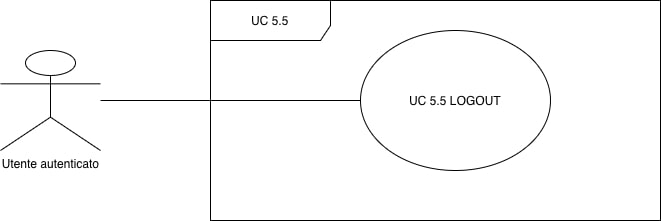
\includegraphics[width=0.8\textwidth]{../UCimg/UC5.3.jpg}
    \caption{Diagramma dei casi d'uso UC-5.3, 5.3.1}
    \label{fig:uc5.3}
\end{figure}

\subsubsection{UC-5.4 - Salvataggio file nel DataBase}
\begin{itemize}
    \item \textbf{Attore principale}: Utente autenticato
    \item \textbf{Descrizione}: L'utente vuole salvare la nota scritta nel database, senza scaricarla nel suo dispositivo corrente
    \item \textbf{Precondizioni}: L'utente ha scritto una nota ed ha eseguito l'accesso al sistema con il suo account
    \item \textbf{Postcondizioni}: Il sistema mantiene nel Database una copia della nota scritta, legandola all'account dell'utente
    \item \textbf{Scenario principale}:
        \begin{itemize}
            \item L'utente accede al sistema
            \item L'utente scrive del testo o ne genera con l'opzione relativa
            \item L'utente seleziona l'opzione di salvataggio
            \item Il sistema salva nel db una copia della nota dell'utente
        \end{itemize}
    \item \textbf{Estensioni}:
        \begin{itemize}
            \item L'utente non ha scritto o generato alcun testo
            \item L'utente non è autenticato
        \end{itemize}
\end{itemize}

\subsubsection{UC-5.4.1 - Gestione tentativo salvataggio nota vuota}
\begin{itemize}
    \item \textbf{Attore principale}: Utente autenticato
    \item \textbf{Descrizione}: Il sistema impedisce il salvataggio di documenti privi di contenuto nel database per evitare record inutili
    \item \textbf{Precondizioni}: L’editor è vuoto e l'utente attiva il comando di salvataggio
    \item \textbf{Postcondizioni}: Il salvataggio viene abortito e l'utente viene avvisato
    \item \textbf{Scenario principale}:
    \begin{itemize}
        \item Il sistema analizza il contenuto dell'editor prima di procedere al salvataggio
        \item Il sistema rileva che non vi è testo o contenuto generato (lunghezza zero o solo spazi bianchi)
        \item Il sistema blocca la procedura di invio al database
        \item Il sistema visualizza un messaggio di avviso
        \item Il documento non viene salvato
    \end{itemize}
\end{itemize}

\subsubsection{UC-5.4.2 - Gestione salvataggio senza autenticazione}
\begin{itemize}
    \item \textbf{Attore principale}: Utente non autenticato (Utente generico)
    \item \textbf{Descrizione}: Il sistema gestisce il tentativo di utilizzare la funzionalità di salvataggio in cloud da parte di un utente non loggato
    \item \textbf{Precondizioni}: L’utente non ha effettuato il login e tenta di salvare su DB
    \item \textbf{Postcondizioni}: Il salvataggio su DB viene negato e vengono proposte alternative
    \item \textbf{Scenario principale}:
    \begin{itemize}
        \item L’utente seleziona l’opzione "Salva nel Database"
        \item Il sistema verifica lo stato della sessione utente
        \item Il sistema rileva che l'utente non è autenticato
        \item Il sistema blocca l'operazione di salvataggio remoto
        \item Il sistema mostra un avviso indicando la necessità di eseguire l'accesso
        \item Il sistema suggerisce all'utente le alternative disponibili
    \end{itemize}
\end{itemize}

\begin{figure}[H]
    \centering
    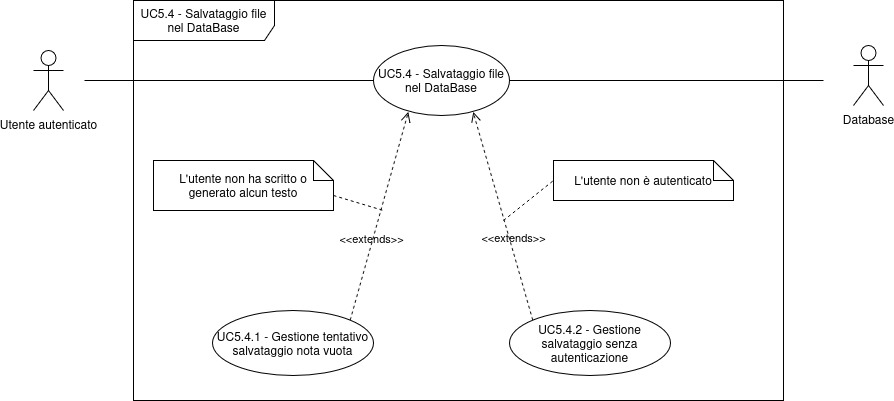
\includegraphics[width=0.8\textwidth]{../UCimg/UC5.4.jpg}
    \caption{Diagramma dei casi d'uso UC-5.4, 5.4.1, 5.4.2}
    \label{fig:uc5.4}
\end{figure}

\subsubsection{UC-5.5 - Logout}
\begin{itemize}
    \item \textbf{Attore principale}: Utente autenticato
    \item \textbf{Descrizione}: L'utente desidera terminare la propria sessione
    \item \textbf{Precondizioni}: L'utente è autenticato nel sistema
    \item \textbf{Postcondizioni}: L'utente viene disconnesso dal sistema
    \item \textbf{Scenario principale}:
        \begin{itemize}
            \item L'utente accede al sistema
            \item L'utente desidera disconnettersi
            \item L'utente seleziona l'opzione "Logout"
            \item L'utente viene disconnesso dal sistema
            \item La sessione dell'utente termina
            \item L'utente viene riportato alla pagina iniziale
        \end{itemize}
\end{itemize}

\begin{figure}[H]
    \centering
    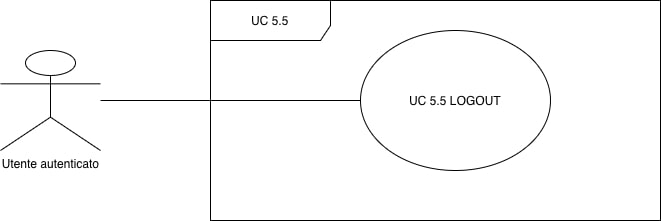
\includegraphics[width=0.8\textwidth]{../UCimg/UC5.5_logout.drawio.jpg}
    \caption{Diagramma del caso d'uso UC-5.5}
    \label{fig:uc5.5}
\end{figure}

\newpage

\section{Requisiti}
\subsection{Classificazione dei requisiti}
Il gruppo ByteMe durante l'analisi dei requisiti e dei casi d'uso ha individuato i requisiti esposti di seguito.
I requisiti sono stati classificati secondo una notazione standardizzata per garantirne la tracciabilità e una chiara comprensione.
Ogni requisito è identificato da un codice univoco che ne esplicita l'importanza e la tipologia.

\subsubsection{Notazione standardizzata dei requisiti}
Il codice identificativo segue il formato:
\[
R[Importanza]-[Tipo]-[Numero]
\]
Dove le voci assumono i seguenti significati:

\begin{description}
    \item[Importanza] \hfill \\
    Indica il grado di priorità del requisito:
    \begin{itemize}
        \item \textbf{O (Obbligatorio):} Requisito esplicitamente richiesto dall'azienda Zucchetti. La sua mancata implementazione implica il fallimento degli obiettivi primari del progetto.
        \item \textbf{D (Desiderabile):} Requisito non strettamente vincolante ma che il gruppo si impegna ad implementare per migliorare il prodotto.
        \item \textbf{OP (Opzionale):} Requisito di priorità minore, la cui implementazione può essere rimandata.
    \end{itemize}
    
    \item[Tipo] \hfill \\
    Indica la natura del requisito:
    \begin{itemize}
        \item \textbf{F (Funzionale):} Descrive le funzionalità e i servizi che il sistema deve fornire.
        \item \textbf{V (Vincolo):} Descrive limitazioni tecnologiche, normative o implementative imposte esternamente.
        \item \textbf{Q (Qualità):} Descrive le caratteristiche qualitative del sistema (es. performance, sicurezza, manutenibilità).
    \end{itemize}
    
    \item[Numero] \hfill \\
    Un numero intero progressivo univoco per tipologia di requisito.
\end{description}

\subsection{Categorie dei Requisiti}
Per una maggiore chiarezza espositiva, i requisiti sono stati suddivisi in tre macro-categorie distinte.

\subsubsection{Requisiti Funzionali}
I requisiti funzionali\textsubscript{G} definiscono i comportamenti specifici del sistema, descrivendo le interazioni tra gli attori e il software.
Rappresentano le funzionalità tangibili che l'utente utilizza per raggiungere i propri obiettivi (es. scrittura del testo, selezione per analisi AI, esportazione documenti). La verifica di tali requisiti determina l'aderenza del prodotto alle funzioni richieste dal capitolato.

\subsubsection{Requisiti Funzionali}
\begin{longtable}{|p{0.2\textwidth}|>{\raggedright\arraybackslash}p{0.5\textwidth}|p{0.2\textwidth}|}
\hline
\textbf{Requisito} & \textbf{Descrizione} & \textbf{Casi d'uso correlati}\\
\hline
\endhead
RO-F-1 & Il sistema deve fornire un editor di testo per l'inserimento e la modifica di caratteri alfanumerici e la compilazione markdown& UC-1.0 \\
\hline
RO-F-2 & L'editor deve compilare la sintassi Markdown in tempo reale & UC-1.1 \\
\hline
RO-F-3 & Deve essere presente un'area di visualizzazione del documento formattato rispetto alla sintassi Markdown & UC-1.1 \\
\hline
RO-F-4 & Il sistema deve permettere all'utente di selezionare porzioni di testo tramite mouse o tastiera & UC-1.2, UC-2.0, UC-2.6, UC-2.7, UC-2.7.*, UC-2.9, UC-2.10, UC-2.11 \\
\hline
RO-F-5 & Il sistema deve permettere all'utente di modificare porzioni di testo selezionate & UC-1.2 \\
\hline
RO-F-6 & Il sistema deve permettere all'utente di copiare una parte di testo selezionato& UC-1.3 \\
\hline
RO-F-7 & Il sistema deve permettere all'utente di incollare una parte del testo & UC-1.4 \\
\hline
RO-F-8 & Il sistema deve permettere all'utente di tagliare di testo selezionato & UC-1.5 \\
\hline
RO-F-9 & Il sistema deve permettere all'utente di annullare l'ultima modifica effettuata & UC-1.6 \\
\hline
RO-F-10 & Il sistema deve permettere all'utente di ripristinare le modifiche precedentemente cancellate & UC-1.7 \\
\hline
RO-F-11 & Nell'editor è presente una barra degli strumenti (toolbar) per applicare formattazioni Markdown senza scrivere manualmente la sintassi & UC-1.8, UC-1.8.* \\
\hline
RO-F-12 & Il sistema deve permettere l'applicazione del grassetto al testo tramite toolbar & UC-1.8.1 \\
\hline
RO-F-13 & Il sistema deve permettere l'applicazione del corsivo al testo tramite toolbar & UC-1.8.2 \\
\hline
RO-F-14 & Il sistema deve permettere l'applicazione della sottolineatura al testo tramite toolbar & UC-1.8.3 \\
\hline
RO-F-15 & Il sistema deve permettere di creare delle intestazioni tramite toolbar & UC-1.8.4 \\
\hline
RO-F-16 & Il sistema deve permettere di modificare la struttura del testo tramite toolbar & UC-1.8.4 \\
\hline
RO-F-17 & Il sistema deve permettere l'inserimento di elementi di struttura (tabelle, separatori) tramite toolbar & UC-1.8.5 \\
\hline
RO-F-18 & Il sistema deve permettere l'inserimento di liste numerate testo tramite toolbar & UC-1.8.6 \\
\hline
RO-F-19 & Il sistema deve permettere l'inserimento di elenchi puntati nel testo tramite toolbar & UC-1.8.6 \\
\hline
RO-F-20 & Il sistema deve permettere l'inserimento di link e riferimenti tramite toolbar & UC-1.8.7 \\
\hline
RO-F-21 & L'utente può applicare più stili (es: grassetto, corsivo, sottolineatura) alla stessa sezione di testo & UC-1.8.* \\
\hline
RO-F-22 & L'utente può annullare una formattazione di una porzione di testo selezionato riselezionandola dalla toolbar & UC-1.8.* \\
\hline
RO-F-23 & L'utente può estendere la formattazione di una porzione di testo selezionato riselezionandola dalla toolbar & UC-1.8.* \\
\hline
RO-F-24 & L'utente può creare sottoliste scegliendo di creare una lista dalla toolbar quando il cursore è già all'interno di una lista  & UC-1.8.6.* \\
\hline
RO-F-25 & L'utente può scegliere una combinazione di opzioni di formattazioni dalla toolbar quando non c'è alcun testo selezionato per applicarle a testo futuro & UC-1.9.* \\
\hline
RO-F-26 & Il sistema deve supportare l'inserimento e la visualizzazione di caratteri Unicode (supporto multilingua) & UC-1.0 \\
\hline
RO-F-27 & Il sistema permette di inviare del testo ad un agente esterno & UC-2.* \\
\hline
RO-F-28 & L'utente deve poter accedere alle azioni sul testo tramite agente esterno in ogni momento & UC-2.0 \\ 
\hline
RO-F-29 & Una volta generato, il testo dell'agente esterno viene inserito nell'editor dal sistema, in modo che tutte le funzionalità dell'editor siano applicabili anche al testo generato & UC-2.* \\
\hline
RO-F-30 & L’utente può modificare, formattare e annullare le generazioni di testo & UC-2.1.* \\
\hline
RO-F-31 & Ogni interazione con un agente esterno che ha come effetto quella di generare del testo, viene inclusa in un registro delle generazioni, anche quelle annullate dall'utente & UC-2.1.4 \\
\hline
RO-F-32 & Il testo generato viene prima mostrato come proposta: ogni proposta viene generata separata dal testo dell'utente & UC-2.1 \\
\hline
RO-F-33 & Il testo in stato di proposta, include le opzioni di conferma, annullamento o rigenerazione & UC-2.1 \\
\hline
RO-F-34 & Il sistema permette la modifica del testo generato in stato di proposta & UC-2.* \\
\hline
RO-F-35 & Una proposta che viene confermata viene inserito nel documento e la sezione di proposta viene rimossa & UC-2.1.1 \\
\hline
RO-F-36 & Una proposta che viene rigenerata viene rimandata all'agente esterno con gli stessi parametri e la nuova risposta sovrascrive la proposta corrente & UC-2.1.4 \\
\hline
RO-F-37 & Una proposta annullata comporta la rimozione del testo generato e della sezione corrispondente & UC-2.1.5 \\
\hline
RO-F-38 & L'utente può consultare il registro delle generazioni effettuate & UC-2.1.6 \\
\hline
RO-F-39 & Il sistema consente all'utente di avviare l'analisi del testo selezionato o dell'intero testo utilizzando il cappello scelto & UC-2.6 \\
\hline
RO-F-40 & Il sistema permette l'invio di un prompt scritto dall'utente per la generazione del testo tramite agente esterno & UC-2.7 \\
\hline
RO-F-41 & Il sistema permette la modifica del prompt da inviare ad un agente esterno & UC-2.6 \\
\hline
RO-F-42 & Il sistema permette di avviare la correzione grammaticale & UC-2.5.* \\
\hline
RO-F-43 & L'utente deve poter riassumere tutto o una parte selezionata del testo usando un agente esterno & UC-2.2 \\
\hline
RO-F-44 &  L'utente deve poter usare un agente esterno per riscrivere tutto o una parte selezionata del testo migliorandolo seguendo determinate specifiche come sintassi, stile e chiarezza & UC-2.3 \\
\hline
RO-F-45 & L'utente deve poter tradurre il testo usando un agente esterno in: inglese, italiano, tedesco, francese, spagnolo e cinese mandarino & UC-2.4.* \\
\hline
RO-F-46 & Se la generazione di testo si blocca prematuramente, rimarrà ciò che è già stato generato, in attesa che l'utente confermi, rigeneri o elimini ciò che è stato generato & UC-2.* \\
\hline
RO-F-47 & L'agente esterno può generare testo basandosi su prompt inviatogli dall'utente & UC-2.7.* \\
\hline
RO-F-48 & L'utente può caricare/aprire un file dal proprio dispositivo all'interno dell'editor & UC-3.* \\
\hline
RO-F-49 & Il sistema deve supportare il caricamento tramite dialogo di esplorazione file (file picker) & UC-3.0.* \\
\hline
RO-F-50 & Il sistema deve permettere all'utente di rimuovere il file che ha caricato (chiudendo il documento o l'editor) & UC-3.3 \\
\hline
RO-F-51 & Prima di procedere con il caricamento di un file, il sistema chiede conferma all'utente & UC-3.0 \\
\hline
RO-F-52 & Il sistema deve consentire l'esportazione del documento in formato PDF. & UC-4.0.1\\
\hline
RO-F-53 & Il sistema deve essere in grado di convertire il documento da Markdown al formato selezionato dall'utente. & UC-4.0 \\
\hline
RO-F-53 & Il sistema deve controllare che il range di pagine inserito dall'utente sia valido (che non superi il numero di pagine presenti o che non sia un numero negativo). & UC-4.1.* \\
\hline
RO-F-54 & Il sistema deve permettere di poter scaricare il file nel dispositivo dell'utente. & UC-4.0\\
\hline
RO-F-55 & Il sistema deve potersi collegare a un dispositivo di stampa. & UC-4.2\\
\hline
RD-F-1 & Il sistema deve supportare l'uso di scorciatoie da tastiera per le operazioni di formattazione & UC-1.8.* \\
\hline
RD-F-2 & Il sistema deve permettere di cambiare modalità di visualizzazione (Solo Editor, Solo Anteprima, Split View) & UC-1.10.* \\
\hline
RD-F-3 & Il sistema deve supportare il caricamento tramite drag-and-drop (trascinamento file nell'area dell'editor) & UC-3.0.1 \\
\hline
RD-F-4 & Il sistema deve offrire opzioni per le operazioni comuni sui file come carica nuovo, stampa, chiudi & UC-1.0 \\
\hline
RD-F-5 & Se sono presenti modifiche non salvate nell'editor, il sistema chiede conferma all'utente prima di caricare un nuovo file, permettendo di annullare l'operazione, per salvare il testo presente, o sovrascrivere il contenuto senza salvarlo & UC-3.0 \\
\hline
RD-F-6 & Il sistema deve consentire l'esportazione del documento in formato MD. & UC-4.0.2 \\
\hline
RD-F-7 & Il sistema deve consentire l'esportazione del documento in formato HTML. & UC-4.0.3 \\
\hline
RD-F-8 & Il sistema deve consentire l'esportazione del documento in formato ODT. & UC-4.0.4 \\
\hline
RD-F-9 & Il sistema deve consentire l'esportazione del documento in formato DOCX. & UC-4.0.5 \\
\hline
RD-F-10 & L'utente deve poter scegliere se esportare l'intero documento, un range di pagine o una quantità selezionata di pagine. & UC-4.1.*\\
\hline
RD-F-11 & Il sistema deve permettere all'utente di scegliere se stampare tutto il documento o una quantità selezionata di pagine. & UC-4.2.*\\
\hline
ROP-F-1 & L'utente può ricercare parole nel testo attraverso l'editor & UC-1.11 \\
\hline
ROP-F-2 & La sezione di testo generata come proposta è visibilmente diversa dal testo utente & UC-2.* \\
\hline
ROP-F-3 & La sezione di testo in stato di proposta viene colorata in base al tipo di operazione che viene fatta & UC-2.0 \\
\hline
ROP-F-4 & Il sistema offre esempi per la richiesta di generazione di testo a partire da un estratto & UC-2.7 \\
\hline
ROP-F-5 & Il sistema permette di inserire un grafico generato, con dati presenti nel testo, scelto tra diversi tipi disponibili all'utente & UC-2.8 \\
\hline
ROP-F-6 & Il sistema permette di inserire una tabella generata con dati presenti nel testo & UC-2.8 \\
\hline
ROP-F-7 & Il sistema permette di inserire una mappa concettuale generata con dati presenti nel testo & UC-2.9 \\
\hline
ROP-F-8 & Il sistema permette di inserire una formula matematica generata con dati presenti nel testo & UC-2.10 \\
\hline
ROP-F-9 & Il sistema deve permettere all'utente di inserire le proprie credenziali (username e password) per il login & UC-5.0 \\
\hline
ROP-F-10 & Se le credenziali sono errate il sistema deve non far autenticare l'utente & UC-5.0.* \\
\hline
ROP-F-11 & Il sistema deve permettere all'utente di potersi registrare tramite uno username e una password & UC-5.1 \\
\hline
ROP-F-12 & Il sistema deve impedire la registrazione in caso ci sia uno username uguale nel database & UC-5.1 \\
\hline
ROP-F-13 & Il sistema deve salvare nel database le password criptate in fase di registrazione & UC-5.1 \\
\hline
ROP-F-14 & Il sistema deve permettere ad un utente autenticato di poter eliminare il proprio account & UC-5.2 \\
\hline
ROP-F-15 & Il sistema in caso di eliminazione account deve eliminare i dati dal database & UC-5.2 \\
\hline
ROP-F-16 & Le operazioni di eliminazione dell'account devono richiedere una conferma esplicita da parte dell'utente & UC-5.2 \\
\hline
ROP-F-17 & Il sistema deve terminare la sessione nel caso un account venga eliminato & UC-5.2 \\
\hline
ROP-F-18 & Il sistema deve permettere ad un utente di vedere i file che ha salvato & UC-5.3 \\
\hline
ROP-F-19 & Il sistema deve permettere ad un utente autenticato di selezionare un file dall'elenco di quelli salvat e aprirlo & UC-5.3 \\
\hline
ROP-F-20 & Il sistema deve consentire all'utente di annullare l'operazione di apertura senza recuperare alcun file dal database & UC-5.3 \\
\hline
ROP-F-21 & Il sistema deve permettere all'utente l'apertura di un file salvato & UC-5.3 \\
\hline
ROP-F-22 & Il sistema deve permettere il salvataggio di un file in un sistema di persistenza non locale & UC-5.4 \\
\hline
ROP-F-23 & Il sistema deve associare ogni file al suo creatore & UC-5.4 \\
\hline
ROP-F-24 & Un utente non autenticato che prova a salvare un file viene riportato alla pagina di login  & UC-5.4.2 \\
\hline
ROP-F-25 & L'utente può effettuare il logout in ogni momento e terminare la propria sessione & UC-5.5 \\

\addlinespace[1em]
\caption{Tabella dei requisiti funzionali}
\end{longtable}

\newpage
\subsubsection{Requisiti di Vincolo}
I requisiti di vincolo\textsubscript{G} rappresentano le limitazioni entro le quali il progetto deve essere sviluppato. A differenza dei requisiti funzionali, questi non derivano da scelte progettuali del team, ma sono imposizioni esterne dettate dal committente, da normative o da limiti tecnologici.
Questi comprendono i vincoli tecnologici, architetturali e organizzativi.

% tabella per i requisiti non funzionali di vincolo
\begin{longtable}{|p{0.2\textwidth}|>{\raggedright\arraybackslash}p{0.5\textwidth}|p{0.2\textwidth}|}
\hline
\textbf{Requisito} & \textbf{Descrizione} & \textbf{Casi d'uso correlati}\\
\hline

RO-V-1 & L'applicazione deve essere accessibile via browser e necessita di connessione internet & UC-1.0 \\
\hline
RO-V-2 & Il sistema deve supportare nativamente la codifica dei caratteri Unicode (UTF-8) per garantire la leggibilità di testi multilingua & UC-1.0 \\
\hline
RO-V-3 & Il formato di input e storage del testo deve essere Markdown & UC-1.0, UC-1.1 \\
\hline
RO-V-4 & L’agente esterno applica modifiche relative esclusivamente al testo selezionato. Un contesto aggiuntivo può essere fornito solo a scopo interpretativo e non deve essere alterato. & UC-2.0 \\
\hline
RO-V-5 & I testi generati dall'agente esterno devono indicare il tipo di operazione che li ha generati nel registro delle generazioni & UC-2.* \\
\hline
RO-V-6 & Il testo generato da un agente esterno che viene accettato dall'utente, viene inserito nella posizione del cursore, se presente nell’editor, altrimenti in fondo al testo & UC-2.* \\
\hline
RO-V-7 & L'agente esterno deve avere istruzioni sufficienti affinché il testo riscritto sia corretto grammaticalmente, sintatticamente e semanticamente e deve riflettere la richiesta dell'utente & UC-2.3 \\
\hline
RO-V-8 & Le sezioni create per la traduzione di un testo specificheranno la lingua di partenza e di fine & UC-2.4.* \\
\hline
RO-V-9 & All'agente esterno devono essere passate delle istruzioni ottimizzate per garantire una traduzione accurata nella lingua selezionata & UC-2.4.* \\
\hline
RO-V-10 & Il sistema espone la sua limitazione nell'eseguire un'azione richiesta se i dati inviati non rispettano i limiti dell'agente esterno & UC-2.9, UC-2.9, UC-2.10 \\
\hline
RO-V-11 & Il caricamento e la lettura del file devono avvenire localmente tramite le API del browser (es. File API), senza inviare il contenuto a un server & UC-3.* \\
\hline
RO-V-12 & L'operazione di esportazione o stampa non deve alterare o chiudere il documento originale nell'editor. & UC-4.* \\
\hline
RO-V-13 & Il sistema deve collegarsi ad un LLM tramite API REST & UC-2.* \\
\hline
RD-V-1 & Il sistema deve supportare l'importazione dei formati di file più comuni: markdown (.md, .markdown) e testo (.txt) & UC-3.0, UC-3.1 \\
\hline
ROP-V-1 & La password inserita dall'utente deve essere minimo 8 caratteri & UC-5.1 \\
\hline
ROP-V-2 & La password inserita dall'utente deve contenere almeno un carattere speciale e un numero & UC-5.1 \\
\hline
ROP-V-3 & L'accesso ai file salvati nel database deve essere consentito solo ad utenti autenticati & UC-5.3 \\
\hline
ROP-V-4 & Il sistema deve impedire il salvataggio di file nel database da parte di utenti non autenticati & UC-5.4 \\
\hline
ROP-V-5 & Se il testo è già nella lingua da tradurre, l'utente viene avvisato e l'operazione viene interrotta & UC-2.4.* \\
\hline
ROP-V-6 & I testi generati dall’agente esterno nel registro delle generazioni devono indicare la data e l’ora della generazione & UC-2.* \\
\hline
\addlinespace[1em]
\caption{Tabella dei requisiti di vincolo}
\end{longtable}


\newpage
\subsubsection{Requisiti di Qualità}
I requisiti di qualità\textsubscript{G} specificano le caratteristiche intrinseche del software. Non descrivono nuove funzioni, ma stabiliscono \textit{come} il sistema deve erogare quelle esistenti. 
% tabella per i requisiti non funzionali di qualità
\begin{longtable}{|p{0.2\textwidth}|>{\raggedright\arraybackslash}p{0.5\textwidth}|p{0.2\textwidth}|}
\hline
\textbf{Requisito} & \textbf{Descrizione} & \textbf{Casi d'uso correlati}\\
\hline

RO-Q-1 & Il sistema deve compilare il testo markdown in un breve lasso di tempo & UC-1.0, UC-1.1 \\
\hline
RO-Q-2 & Il sistema deve fornire messaggi di errore chiari se l'editor non risponde o se l'anteprima fallisce & UC-1.0, UC-1.1 \\
\hline
RO-Q-3 & L'aggiornamento dell'anteprima compilata deve avvenire automaticamente quando viene modificato del testo& UC-1.0, UC-1.1 \\
\hline
RO-Q-4 & Il sistema deve avvisare l'utente in caso di mancanza di connessione & UC-1.0 \\
\hline
RO-Q-5 & Il sistema deve avvisare l'utente se l'editor non risponde & UC-1.0 \\
\hline
RO-Q-6 & Il sistema deve avvisare l'utente se l'anteprima non si aggiorna & UC-1.1 \\
\hline
RO-Q-7 & Il sistema non fa niente se non ci sono azioni da annullare & UC-1.6 \\
\hline
RO-Q-8 & Il sistema non fa niente se non ci sono azioni da ripetere & UC-1.7 \\
\hline
RO-Q-9 & Il sistema esplicita se la ricerca non ha prodotto risultati & UC-1.11 \\
\hline
RO-Q-10 & L'agente esterno deve rispondere sempre in tempi brevi, o restituire errore & UC-2.* \\
\hline
RO-Q-11 & Il sistema deve intercettare e gestire gli errori di comunicazione con il servizio LLM. & UC-2.* \\
\hline
RO-Q-12 & Le opzioni, relative alle operazioni con agente esterno, non devono sparire in maniera poco intuitiva muovendo il mouse & UC-2.0 \\
\hline
RO-Q-13 & Il sistema mostra un messaggio in caso di errore durante la generazione di contenuto & UC-2.* \\
\hline
RO-Q-14 & Il sistema deve fornire un feedback visivo immediato all'utente (messaggio di errore o di successo) al termine del tentativo di caricamento file & UC-3.* \\
\hline
RO-Q-15 & Il sistema deve validare il formato del file caricato e impedire il caricamento di formati non supportati & UC-3.1 \\
\hline
RO-Q-16 & Il sistema deve validare le dimensioni del file caricato e impedire il caricamento di file che superano una dimensione massima & UC-3.2 \\
\hline
RO-Q-17 & Il sistema deve impedire il caricamento di file corrotti & UC-3.0, UC-3.1\\
\hline
RO-Q-18 & La dimensione massima consentita per il caricamento di un file deve essere limitata a una soglia definita e ragionevole & UC-3.2 \\
\hline
RO-Q-19 & Il sistema deve avvisare l'utente della buona riuscita o di eventuali errori durante il download. & UC-4.0 \\
\hline
RO-Q-20 & Il sistema deve avvisare l'utente in caso di errore durante l'invio del documento alla stampante. & UC-4.2 \\
\hline
RO-Q-21 & Il sistema deve poter permettere di visualizzare sia il testo in lingua originale che la traduzione generata & UC-2.5, UC-2.5.x \\
\hline
RD-Q-1 & I messaggi di errore (per formato errato, file troppo grande o corrotto) devono essere esplicativi e suggerire all'utente come procedere & UC-3.* \\
\hline
RD-Q-2 & L'operazione di caricamento e rendering di un file di dimensioni supportate deve completarsi in tempi brevi & UC-3.0.*\\
\hline
RD-Q-3 & Il parsing del contenuto del file deve essere robusto, garantendo che caratteri non validi non causino il crash dell'applicazione & UC-3.* \\
\hline
RD-Q-4 & Il sistema deve fornire una visualizzazione in anteprima del documento nel formato selezionato prima di procedere al download. & UC-4.0 \\
\hline
RD-Q-5 & Il sistema deve permettere all'utente di scegliere il nome del file prima di scaricare il documento. & UC-4.0 \\
\hline
ROP-Q-1 & Il sistema deve mostrare un messaggio di errore non specifico nel caso di fallimento del login & UC-5.0 \\
\hline
ROP-Q-2 & Il sistema deve avvisare l'utente che lo username è già stato usato & UC-5.1 \\
\hline
ROP-Q-3 & Il sistema propone all'utente di effettuare il login o scegliere un nuovo username & UC-5.1 \\
\hline
ROP-Q-4 & Il sistema mostra i file salvati in ordine cronologico & UC-5.3 \\
\hline
ROP-Q-5 & Il sistema deve notificare all'utente il fallimento del salvataggio & UC-5.4 \\
\hline
\addlinespace[1em]
\caption{Tabella dei requisiti di qualità}
\end{longtable}

\newpage

\section{Riepilogo}
\begin{table}[H]
\centering
\begin{tabular}{|p{0.2\textwidth}|>{\raggedright\arraybackslash}p{0.1\textwidth}|p{0.1\textwidth}|p{0.1\textwidth}|p{0.1\textwidth}|}
\hline
\textbf{Tipologia} & \textbf{O} & \textbf{D} & \textbf{OP} & \textbf{Totale}\\
\hline
Funzionali & 43 & 11 & 25 & 79 \\
\hline
Vincolo & 12 & 1 & 5 & 18 \\
\hline
Qualità & 15 & 6 & 5 & 26 \\
\hline
\textbf{Totale} & 70 & 18 & 35 & 123\\
\hline
\end{tabular}
\caption{Riepilogo dei requisiti}
\end{table}

\end{document}
